\documentclass[xcolor={usenames,dvipsnames}]{beamer}
%
% ugly hack referring to the slides folder. Works for me.
%
\makeatletter
\def\input@path{{/Users/denilson/teaching/cmput391/git-slides/}}
\makeatother

% \usepackage[T1]{fontenc} % font encoding
% \usepackage{fontspec}
\usepackage{fontspec}


\makeatletter%
\@ifclassloaded{beamer}{%
  \usepackage{lmodern} %%% modern beamer style
  %%beamer style
  \usetheme{metropolis}
  \usefonttheme{professionalfonts}
  \setbeamercolor{background canvas}{bg=background}
  \setbeamercolor{frametitle}{bg=snow,fg=black}
  \setbeamercolor{title separator}{fg=snow}
  \setbeamercolor{alerted text}{fg=accent}

  \let\oldtitle\title
  \renewcommand{\title}[1]{\oldtitle{CMPUT391\\#1}}
  \author{Instructor: Denilson Barbosa}
  \date{\small University of Alberta}
  \institute{\today\vskip4em Slides by D. Barbosa, with suggested corrections and improvements by (in alphabetical order) C. Bins, D. Caminhas, K. Guhzva, Q. Lautischer, E. Macdonald, M. A. Nascimento, K. Newbury, M. Strobl, D. Sunderman, K. Wang, and K. Wong.}
  
  \titlegraphic{\includegraphics[width=1.5cm]{../images/by-sa.png}~
  {\tiny This work is licensed under a Creative Commons Attribution 4.0 International License}}

  %%%% un-framed blocks
  \setbeamertemplate{blocks}[rounded][shadow=false]
}{}

\@ifpackageloaded{xcolor}{}{
  \usepackage{xcolor}
}
\makeatother


\setsansfont[BoldFont={Open Sans SemiBold}]{Open Sans}[Scale=0.85]
\setmonofont{Cousine}[Scale=0.8]
\setmathtt{Cousine}[Scale=0.8]

%%%% highlighting text 
\usepackage{xspace}
\def\highlight#1{\colorbox{accent}{\textcolor{white}{#1}}\xspace}

\def\blue#1{\textcolor{blue}{#1}}

%
%
%
\usepackage{parskip}

\usepackage{subcaption} % needed for subfigures

\usepackage{wrapfig} % for figures "to the side of the text"

\usepackage{anyfontsize} % for egregious warnings

%
% Fonts
%
% \usepackage{amsmath}
% \usepackage{mathspec}
% \setmathtt[Scale=0.875]{Cousine}

%
% various packages for tables and colored tables
%
\usepackage{xcolor,colortbl}
\usepackage{tcolorbox}

\definecolor{accent}{RGB}{225,68,85}
\definecolor{highlight}{RGB}{170,68,153}
\definecolor{background}{rgb}{253,252,252}

\definecolor{sqlColor}{RGB}{119,119,17}

\definecolor{Cfunction}{RGB}{51,51,153}

\definecolor{stringColor}{RGB}{51,51,153}
\definecolor{datatypeColor}{RGB}{170,68,153}
\definecolor{functionColor}{RGB}{51,134,116}

\definecolor{exampleColor}{RGB}{51,34,136}
\definecolor{commentColor}{RGB}{112,68,225}

\definecolor{fern}{RGB}{80,118,66}

\definecolor{snow}{RGB}{240,240,230}
\definecolor{Gray}{gray}{0.85}

\definecolor{tupleBoxColor}{gray}{0.85}

\definecolor{Maroon}{RGB}{139,0,0}

%
% coloring of SQL code
%
\def\ColorSymbol#1{\textcolor{functionColor}{#1}}

%
% hihglight box
%
\usepackage{xspace}
\def\highlight#1{\colorbox{accent}{\textcolor{white}{#1}}\xspace}

%
% Tables
%
\usepackage{multirow}
\usepackage{multicol}

%
% CODE LISTINGS
%
\usepackage{listings}

%
% catch-all style meant to provide a clean and "empty" style
% from which all others build upon
%
\lstdefinestyle{cmput391}{
  style=,
  frame=no,
  tabsize=2,
  numbers=none,
  showstringspaces=false,
  numberstyle=\footnotesize,
  basicstyle=\ttfamily\footnotesize\color{black},
  numbersep=4pt,
  keywords=[1]{},
  keywords=[2]{},
  keywords=[3]{sh_lock,xl_lock,unlock,read,write,commit,abort},
  keywordstyle=[1]\ttfamily\bfseries\footnotesize,
  keywordstyle=[2]\ttfamily\footnotesize,
  keywordstyle=[3]\ttfamily\footnotesize\color{Maroon},
  emph=[1]{},
  emph=[2]{},
  emph=[3]{},
  emphstyle=[1]\ttfamily\footnotesize,
  emphstyle=[2]\ttfamily\footnotesize,
  emphstyle=[3]\ttfamily\footnotesize,
  commentstyle=\ttfamily\itshape\color{commentColor},
  stringstyle=\ttfamily\color{stringColor},
  moredelim=**[l][\itshape\color{commentColor}]{--},
  moredelim=**[is][\color{highlight}]{-|}{|-},
  moredelim=[is][\bfseries\color{highlight}]{-:}{:-},
  morestring=[s][\color{stringColor}]{"}{"},
  morecomment=[l]{--}
}

\lstdefinelanguage{DTD}{
  style=cmput391,
  morekeywords=[1]{DOCTYPE,ELEMENT,ATTLIST},
  keywordstyle=[1]\color{accent},
  literate = {\#PCDATA}{{\textcolor{Cfunction}{\#PCDATA}}}7
             {\#IMPLIED}{{\textcolor{Cfunction}{\#IMPLIED}}}8
}

\lstdefinelanguage{XPath}{
  style=cmput391,
  morekeywords={xs,integer,current,date,distinct,values,avg,text,id,count,position,and,or,not,boolean,number,sum,floor,ceiling,round,doc,eq,ne,gt,lt,ge,le},
  keywordstyle=\color{red},
  literate = {last(}{{\textcolor{functionColor}{last}(}}5 {@<}{{<}}1  
}

\lstdefinestyle{XQuery}{
  style=cmput391,
  keywords=[1]{if,then,else,and,or,some,every,satisfies,for,in,let,where,group,order,by,return,ascending},
  keywords=[2]{gt,lt,eq,ne,ge,le,not,or},
  keywords=[3]{text,sum,min,max,avg,len,position,number,boolean,floor,ceiling,round,%
               id,doc,count,current-date,distinct-values,xs:integer,subsequence},
  keywordstyle=[1]\bfseries\color{sqlColor},
  keywordstyle=[2]\color{accent},
  keywordstyle=[3]\color{functionColor},
  moredelim =[is][\color{blue}]{-:}{:-},
  moredelim =[s][\color{accent}]{<}{>},
  moredelim=**[s][\color{black}]{/}{\ },
  moredelim=*[s][\color{blue}]{\$}{\ },
  alsoletter=:{:,-},
  literate = {(}{{\textcolor{black}{(}}}{1} {)}{{\textcolor{black}{)}}}{1} 
             {\{}{{\textcolor{black}{\{}}}{1} {\}}{{\textcolor{black}{\}}}}{1} 
             {last(}{{\textcolor{functionColor}{last}(}}5 {@<}{{<}}1
}


\lstdefinestyle{SQL}{
  style=cmput391,
  language=SQL,
  sensitive={True},
  deletekeywords={year,Cast,MIN,MAX},
  morekeywords={ABORT,AFTER,BEFORE,REFERENCES,REFERENCING,WITH,COMMITTED,UNCOMMITTED,REPEATABLE,SERIALIZABLE},
  keywords=[2]{AVG,MIN,MAX,COUNT,SUM,NEW,OLD,strftime,date,length,RAISE,rowid,substr},
  keywords=[3]{BIGINT,CHAR,DATE,DECIMAL,INT,FLOAT,TEXT},
  keywordstyle=[1]\ttfamily\bfseries\color{sqlColor},
  keywordstyle=[2]\ttfamily\bfseries\color{functionColor},
  keywordstyle=[3]\ttfamily\bfseries\color{datatypeColor},
  moredelim=**[is][\ttfamily\bfseries\color{functionColor}]{(@}{@)},
  morestring=[s][\color{stringColor}]{'}{'},
  moredelim=[is][\bfseries\color{highlight}]{-:}{:-}
}


%
% lstlisting for command line examples
%
\lstdefinestyle{commandLine}{
  basicstyle=cmput391,
  keywordstyle=[1]\ttfamily\bfseries\color{functionColor},
  keywordstyle=[2]\ttfamily\bfseries\color{datatypeColor},
  moredelim=**[is][\color{accent}\bf]{@}{@}
  keywords=[1]{%
    grep},
  keywords=[2]{%
    postings}
}

%
% lstlisting for C code
%
\lstdefinestyle{C}{
  language=C,
  tabsize=2,
  basicstyle=\ttfamily\footnotesize,
  stringstyle=\color{stringColor},
  keywords=[2]{sqlite3_prepare_v2,sqlite3_bind_int64,sqlite3_step,sqlite3_exec},
  keywordstyle=[1]\ttfamily\bfseries\color{datatypeColor},
  keywordstyle=[2]\ttfamily\bfseries\color{functionColor},
  commentstyle=\ttfamily\itshape\color{commentColor},
  moredelim=**[is][\color{Cfunction}\bf\ttfamily]{@}{@}
}


\lstdefinestyle{Python}{
  language=Python,
  tabsize=2,
  basicstyle=\ttfamily\footnotesize,
  stringstyle=\color{stringColor},
  morekeywords=[1]{self,yield,Class,true,false,None},
  keywords=[2]{satisfies,from,Iterator,EOF,concatenate,advance,join,rewind},
  deletekeywords=[1]{from},
  keywordstyle=[1]\ttfamily\bfseries\color{datatypeColor},
  keywordstyle=[2]\ttfamily\bfseries\color{functionColor},
  commentstyle=\ttfamily\itshape\color{commentColor},
  moredelim=**[is][\color{Cfunction}\bf\ttfamily]{@}{@}
}



%
% lstlisting style for RDF/SPARQL
%
\lstdefinestyle{SPARQL}{
  style=cmput391,
  sensitive={True},
  keywords=[1]{BASE,PREFIX,SELECT,WHERE,FILTER,MINUS,NOT,EXISTS},
  keywordstyle=[1]\ttfamily\bfseries\color{sqlColor},
  moredelim=*[s][\color{Cfunction}]{?}{\ },
  moredelim=*[s][\color{Cfunction}]{@}{\ },
  morestring=[s][\color{datatypeColor}]{"}{"},
  literate =* {|}{{|}}1 {//}{{//}}2 {< }{< }{2}
}

%
% coloring of markup code
%
\lstdefinestyle{markup}{
  style=cmput391,
  literate =* {=}{{\color{sqlColor}{=}}}1,
  moredelim =* [s][\color{accent}]{<}{>},
  moredelim =** [is][\color{accent}]{@}{@},
  moredelim =** [is][\color{blue}]{-:}{:-},
  morecomment=[s]{<!--}{-->}
}

\lstdefinestyle{RDF}{
  style=cmput391,
  keywords=[1]{BASE,PREFIX},
  keywordstyle=[1]\ttfamily\bfseries\color{functionColor},
  alsoletter=:{:,-,@},
  literate = {prefix}{{\bfseries\textcolor{functionColor}{prefix}}}6 
             {:}{{\textcolor{functionColor}{:}}}1 
             {@}{{\textcolor{functionColor}{@}}}1,
  moredelim =* [s][\color{accent}]{<}{>},
  moredelim =** [is][\color{functionColor}]{-:}{:-},
  morecomment=[s]{<!--}{-->}
}




















%
% Tikz stuff, for cummulative diagrams and algebra trees
%
\usepackage{tikz} %commutative diagrams
\usepackage{tikz-cd} %commutative diagrams
\usetikzlibrary{positioning}% To get more advances positioning options
\usetikzlibrary{arrows,shapes,automata}
\usetikzlibrary{calc} % for calculations and hard-coded coordinates
\usetikzlibrary{tikzmark, fit, shapes.misc}
\usetikzlibrary{decorations.pathreplacing}
\usetikzlibrary{backgrounds} % to draw underneath other elements
\usepackage{stackengine} % to overlay tikz pictures over other things

\usepackage{pgfplots}
\pgfplotsset{compat=1.17}

%
%
% PGF arrowtip that looks like an X
%
%
\pgfarrowsdeclare{X}{X}
{
  \arrowsize=0.25pt
  \advance\arrowsize by .5\pgflinewidth
  \pgfarrowsleftextend{-4\arrowsize-.5\pgflinewidth}
  \pgfarrowsrightextend{.5\pgflinewidth}
}
{
  \arrowsize=0.2pt
  \advance\arrowsize by .5\pgflinewidth
  \pgfsetdash{}{0pt} % do not dash
  \pgfsetroundjoin   % fix join
  \pgfsetroundcap    % fix cap
  \pgfpathmoveto{\pgfpointorigin}
  \pgfpathlineto{\pgfpoint{-5\arrowsize}{5\arrowsize}}
  \pgfusepathqstroke
  \pgfpathmoveto{\pgfpointorigin}
  \pgfpathlineto{\pgfpoint{5\arrowsize}{-5\arrowsize}}
  \pgfusepathqstroke
  \pgfpathmoveto{\pgfpointorigin}
  \pgfpathlineto{\pgfpoint{-5\arrowsize}{-5\arrowsize}}
  \pgfusepathqstroke
  \pgfpathmoveto{\pgfpointorigin}
  \pgfpathlineto{\pgfpoint{5\arrowsize}{5\arrowsize}}
  \pgfusepathqstroke
}


%
%%% for algorithms and pseudocode
%
\usepackage{algorithm}
% \usepackage{algpseudocode}
\usepackage[noend]{algpseudocode}
\renewcommand{\algorithmicrequire}{\textbf{Input:}}
\renewcommand{\algorithmicensure}{\textbf{Output:}}
\algnewcommand\algorithmicforeach{\textbf{for each}}
\algdef{S}[FOR]{ForEach}[1]{\algorithmicforeach\ #1\ \algorithmicdo}
% style for comments inside algorithms
\renewcommand{\algorithmiccomment}[1]{\hspace*{1em}\textcolor{commentColor}{\%~\textit{#1}}} 

%
% to create boxes with verbatim and code-like content
%
\usepackage{verbatimbox}

%
% to crop/trim boxes!
%
\usepackage{trimclip}

%
% colored and framed boxes
%
\newenvironment{BOX}[1]{\begin{tcolorbox}[colback=snow!25,colframe=snow!40!black,title=#1]\small}{\end{tcolorbox}}



%
% math and symbols
%
\usepackage{mathtools}
\DeclarePairedDelimiter{\ceil}{\lceil}{\rceil}
\DeclarePairedDelimiter{\floor}{\lfloor}{\rfloor}
\usepackage{amsbsy} 
\usepackage{amssymb}
\usepackage{ifsym} % needed to produce the common outerjoin symbols

%
% for nice-looking enumerations and inlined enumerations
%
\usepackage[shortlabels,inline]{enumitem}



%%% outer join symbols
\newcommand\TextbookOuterJoin{%
  \mathrel{\ooalign{\hss$\Join$\hss\cr%
  \kern0.5ex\raise1ex\hbox{\scalebox{0.7}{$\circ$}}}}}

\newcommand\RightOuterJoin{%
  \mathrel{%
  	\ooalign{%
  		$\Join$\cr\kern1.25ex\raise0.0975ex\hbox{\scalebox{0.25}[0.8275]{$\sqsubset$}}}
  	}
}

\newcommand\LeftOuterJoin{%
  \mathrel{%
  	\ooalign{%
  		$\Join$\cr\kern-0.0125ex\raise0.0975ex\hbox{\scalebox{0.25}[0.8275]{$\sqsupset$}}}%
	}
}

\newcommand\FullOuterJoin{%
  \mathrel{%
  	\ooalign{%
  		$\Join$\cr\kern-0.0125ex\raise0.0975ex\hbox{\scalebox{0.25}[0.8275]{$\sqsupset$}}}%
  		\kern-0.45ex\raise0.0975ex\hbox{\scalebox{0.25}[0.8275]{$\sqsubset$}}
	}
}






\title{SQL: Review and Recursion}

\begin{document}


% full relational schema

\newsavebox\FullMovieSchema
\begin{lrbox}{\FullMovieSchema}\begin{minipage}{\textwidth}
\begin{lstlisting}[style=SQL]
CREATE TABLE Movie (title CHAR(20), year INT, imdb FLOAT,
   PRIMARY KEY (title, year), CHECK(imdb >= 0 AND imdb <= 10));
CREATE TABLE Director (name CHAR(20), PRIMARY KEY (name));
CREATE TABLE Actor (name CHAR(20), PRIMARY KEY (name));
CREATE TABLE Cinema (name CHAR(20), address CHAR(100), 
   PRIMARY KEY(name));

CREATE TABLE MovieDirector (title CHAR(20), year INT, name CHAR(20)
  PRIMARY KEY (title, year, name),
  FOREIGN KEY (title, year) REFERENCES Movie(title, year),
  FOREIGN KEY (name) REFERENCES Director(name));

CREATE TABLE Cast (title CHAR(20), year INT, name CHAR(20), role CHAR(20), 
  PRIMARY KEY (title, year, name, role),
  FOREIGN KEY (title, year) REFERENCES Movie(title, year)
  FOREIGN KEY (name) REFERENCES Actor(name));

CREATE TABLE Guide (theater CHAR(20), film CHAR(20), year INT, start INT, 
  PRIMARY KEY (theater, film, year, start),
  FOREIGN KEY (theater) REFERENCES Cinema(name), 
  FOREIGN KEY (film, year) REFERENCES Movie(title, year));
\end{lstlisting}
\end{minipage}
\end{lrbox}


% simplified relational schema

\newsavebox\SimplifiedMovieSchema
\begin{lrbox}{\SimplifiedMovieSchema}\begin{minipage}{\textwidth}
\begin{lstlisting}[style=SQL]
CREATE TABLE Movie (title CHAR(20), year INT, imdb FLOAT, 
   director CHAR(20) NOT NULL, PRIMARY KEY (title, year), 
   CHECK(imdb >= 0 AND imdb <= 10));

CREATE TABLE Cinema (name CHAR(20), address CHAR(100), 
   PRIMARY KEY(name));

CREATE TABLE Cast (title CHAR(20), year INT, 
   actor CHAR(20) NOT NULL, role CHAR(20) NOT NULL, 
   FOREIGN KEY (title, year) REFERENCES Movie(title, year));

CREATE TABLE Guide (theater CHAR(20), film CHAR(20), year INT, start INT, 
  PRIMARY KEY (theater, film, year, start),
  FOREIGN KEY (theater) REFERENCES Cinema(name), 
  FOREIGN KEY (film, year) REFERENCES Movie(title, year));
\end{lstlisting}
\end{minipage}
\end{lrbox}

% simplified CREATE MOVIE example

\newsavebox\SimplifiedMovieTableDDL
\begin{lrbox}{\SimplifiedMovieTableDDL}\begin{minipage}{0.9\textwidth}
\begin{lstlisting}[style=SQL]
CREATE TABLE Movie (title CHAR(20), year INT, imdb FLOAT, 
   director CHAR(20), PRIMARY KEY (title, year), 
   CHECK(imdb >= 0 AND imdb <= 10));
\end{lstlisting}
\end{minipage}
\end{lrbox}

% simplified CREATE CAST example

\newsavebox\SimplifiedCastTableDDL
\begin{lrbox}{\SimplifiedCastTableDDL}\begin{minipage}{\textwidth}
\begin{lstlisting}[style=SQL]
CREATE TABLE Cast (title CHAR(20), year INT, 
   actor CHAR(20), role CHAR(20), 
   FOREIGN KEY (title, year) REFERENCES Movie(title, year);
\end{lstlisting}
\end{minipage}
\end{lrbox}
%
% this file has latex "boxes" with each of the tables
% and query results for the examples involving the
% movies database
%

\newsavebox{\MovieTable}
\savebox{\MovieTable}{%
\scriptsize%
\begin{tabular}{l | l | c | l }
\multicolumn{4}{l}{\textbf{Movie}}\\
\hline
\rowcolor{Gray}
\textbf{title} & \textbf{year} & \textbf{imdb} & \textbf{director} \\
\hline
Ghostbusters & 1984 & 7.8 & Ivan Reitman \\
\hline
Big & 1988 & 7.3 & Penny Marshall \\
\hline
Lost in Translation & 2003 & 7.8 & Sofia Coppola \\
\hline
Wadjda & 2012 & 8.1 & Haifaa al-Mansour \\
\hline
Ghostbusters & 2016 & 5.3 & Paul Feig \\
\hline
\end{tabular}
}

\newsavebox{\MovieTableTWO}
\savebox{\MovieTableTWO}{%
\scriptsize%
\begin{tabular}{l | l | c | l }
\multicolumn{4}{l}{\textbf{Movie}}\\
\hline
\rowcolor{Gray}
\textbf{title} & \textbf{year} & \textbf{imdb} & \textbf{director} \\
\hline
Lost in Translation & 2003 & 7.8 & Haifaa al-Mansour \\ % fake tuple :)
\hline
Groundhog day & 1993 & 8 & Harold Ramis \\
\hline
\end{tabular}
}


\newsavebox{\CinemaTable}
\savebox{\CinemaTable}{%
\scriptsize%
\begin{tabular}{l | l }
\multicolumn{2}{l}{\textbf{Cinema}}\\
\hline
\rowcolor{Gray}
\textbf{name} & \textbf{address}  \\
\hline
Garneau & 8712 109 St, Edmonton \\
\hline
Princess & 10337 82 Ave, Edmonton \\
\hline
Landmark & 10200 102 Ave, Edmonton\\
\hline
\end{tabular}
}

\newsavebox{\GuideTable}
\savebox{\GuideTable}{%
\scriptsize%
\begin{tabular}{l | l | l | l }
\multicolumn{4}{l}{\textbf{Guide}}\\
\hline
\rowcolor{Gray}
\textbf{theater} & \textbf{film} & \textbf{year} & \textbf{start}  \\
\hline
Garneau & Ghostbusters & 1984 & 1140 \\
\hline
Garneau & Ghostbusters & 2016 & 1290 \\
\hline
Princess & Wadjda & 2012 & 1260 \\
\hline
\end{tabular}
}


\newsavebox{\CastTable}
\savebox{\CastTable}{%
\scriptsize%
\begin{tabular}{l | l | l | l }
\multicolumn{4}{l}{\textbf{Cast}}\\
\hline
\rowcolor{Gray}
\textbf{title} & \textbf{year} & \textbf{actor} & \textbf{role}  \\
\hline
Ghostbusters & 1984 & Bill Murray & Dr. Venkman \\
\hline
Ghostbusters & 1984 & Sigourney Weaver & Dana Barret \\
\hline
Big & 1988 & Tom Hanks & Josh \\
\hline
Big & 1988 & Elisabeth Perkins & Susan \\
\hline
Lost in Translation & 2003 & Bill Murray & Bob Harris \\
\hline
Wadjda & 2012 & Waad Mohammed & Wadjda \\
\hline
Ghostbusters & 2016 & Dan Aykroyd & Cabbie \\
\hline
Ghostbusters & 2016 & Sigourney Weaver & Dana Barret \\
\hline
\end{tabular}
}

%
% box with all tables together.
%
%%%% NEED TO FIND A NICER WAY THAN THIS...
\newsavebox{\FullInstance}
\savebox{\FullInstance}{%
	\begin{tabular}{@{}l@{}}
		\resizebox{0.6\textwidth}{!}{\usebox{\MovieTable}}\\
		~\\[-0.5em]
		\resizebox{0.7\textwidth}{!}{\usebox{\CastTable}}\\
		~\\[-0.5em]
		\resizebox{0.95\textwidth}{!}{\usebox{\CinemaTable}~~~\usebox{\GuideTable}
		}%
	\end{tabular}%
}

%
% example movie column-oriented store
%
\newsavebox{\MovieTableColTitle}
\savebox{\MovieTableColTitle}{%
\scriptsize%
\begin{tabular}{l | l}
\hline
\rowcolor{Gray}
\ColorSymbol{\textbf{id}} &\textbf{title} \\
\hline
\ColorSymbol{1} & Ghostbusters \\
\hline
\ColorSymbol{2} & Big \\
\hline
\ColorSymbol{3} & Lost in Translation \\
\hline
\ColorSymbol{4} & Wadjda \\
\hline
\ColorSymbol{5} & Ghostbusters \\
\hline
\end{tabular}
}

\newsavebox{\MovieTableColYear}
\savebox{\MovieTableColYear}{%
\scriptsize%
\begin{tabular}{l | l }
\hline
\rowcolor{Gray}
\ColorSymbol{\textbf{id}} &\textbf{year} \\
\hline
\ColorSymbol{1} & 1984 \\
\hline
\ColorSymbol{2} & 1988 \\
\hline
\ColorSymbol{3} & 2003 \\
\hline
\ColorSymbol{4} & 2012 \\
\hline
\ColorSymbol{5} & 2016 \\
\hline
\end{tabular}
}

\newsavebox{\MovieTableColIMDB}
\savebox{\MovieTableColIMDB}{%
\scriptsize%
\begin{tabular}{l | l}
\hline
\rowcolor{Gray}
\ColorSymbol{\textbf{id}} &\textbf{imdb} \\
\hline
\ColorSymbol{1} & 7.8 \\
\hline
\ColorSymbol{2} & 7.3 \\
\hline
\ColorSymbol{3} & 7.8 \\
\hline
\ColorSymbol{4} & 8.1 \\
\hline
\ColorSymbol{5} & 5.3 \\
\hline
\end{tabular}
}

\newsavebox{\MovieTableColDirector}
\savebox{\MovieTableColDirector}{%
\scriptsize%
\begin{tabular}{l | l}
\hline
\rowcolor{Gray}
\ColorSymbol{\textbf{id}} &\textbf{director} \\
\hline
\ColorSymbol{1} & Ivan Reitman \\
\hline
\ColorSymbol{2} & Penny Marshall \\
\hline
\ColorSymbol{3} & Sofia Coppola \\
\hline
\ColorSymbol{4} & Haifaa al-Mansour  \\
\hline
\ColorSymbol{5} & Paul Feig \\
\hline
\end{tabular}
}


%
% Table with selection on Cast.actor='Bill Murray'
%
\newsavebox{\BillMurrayMovies}
\savebox{\BillMurrayMovies}{%
\scriptsize%
\begin{tabular}{l | l | l | l }
\rowcolor{Gray}
\hline
\textbf{title} & \textbf{year} & \textbf{actor} & \textbf{role}  \\
\hline
Ghostbusters & 1984 & Bill Murray & Dr. Venkman \\
\hline
Lost in Translation & 2003 & Bill Murray & Bob Harris \\
\hline
\end{tabular}
}

%
% Table with projection of director on Movie
%
\newsavebox{\MovieDirectors}
\savebox{\MovieDirectors}{%
\scriptsize%
\begin{tabular}{l }
\rowcolor{Gray}
\hline
\textbf{director}  \\
\hline
Ivan Reitman \\
\hline
Penny Marshall \\
\hline
Sofia Coppola \\
\hline
Haifaa al-Mansour  \\
\hline
Paul Feig \\
\hline
\end{tabular}
}

%
% Table with Movie \bowtie \sigma Cast.actor='Bill Murray'
%
\newsavebox{\JoinMoviesBillMurrayMovies}
\savebox{\JoinMoviesBillMurrayMovies}{%
\scriptsize%
\begin{tabular}{l | l | c | l | l | l }
\rowcolor{Gray}
\hline
\textbf{title} & \textbf{year} & \textbf{imdb} & \textbf{director} & \textbf{actor} & \textbf{role}  \\
\hline
Ghostbusters & 1984 & 7.8 & Ivan Reitman & Bill Murray & Dr. Venkman \\
\hline
Lost in Translation & 2003 & 7.8 & Sofia Coppola & Bill Murray & Bob Harris \\
\hline
\end{tabular}
}

%
% Left Outer Join of Cinema and Guide
%
\newsavebox{\LeftOuterJoinCinemaGuide}
\savebox{\LeftOuterJoinCinemaGuide}{%
\scriptsize%
\begin{tabular}{l | l | l | l | l | l}
\hline
\rowcolor{Gray}
\textbf{name} & \textbf{address} & \textbf{theater} & \textbf{film} & \textbf{year} & \textbf{start} \\
\hline
Garneau & 8712 109 St, Edmonton & Garneau & Ghostbusters & 1984 & 1140 \\
\hline
Garneau & 8712 109 St, Edmonton & Garneau & Ghostbusters & 2016 & 1290 \\
\hline
Princess & 10337 82 Ave, Edmonton & Princess & Wadjda & 2012 & 1260 \\
\hline
Landmark & 10200 102 Ave, Edmonton & NULL & NULL & NULL & NULL\\
\hline
\end{tabular}
}

%
% Semijoin of Cinema and Guide
%
\newsavebox{\SemijoinCinemaGuide}
\savebox{\SemijoinCinemaGuide}{%
\scriptsize%
\begin{tabular}{l | l }
\hline
\rowcolor{Gray}
\textbf{name} & \textbf{address}  \\
\hline
Garneau & 8712 109 St, Edmonton \\
\hline
Princess & 10337 82 Ave, Edmonton \\
\hline
\end{tabular}
}

%
% Single tuple in self-join of Cast to get actors in reruns
%
\newsavebox{\SelfJoinExampleSigourneyWeaver}
\savebox{\SelfJoinExampleSigourneyWeaver}{%
\scriptsize%
\begin{tabular}{l | l | l | l | l | l | l | l}
\hline
\rowcolor{Gray}
\textbf{title} & \textbf{year} & \textbf{actor} & \textbf{role}  & \textbf{title2} & \textbf{year2} & \textbf{actor2} & \textbf{role2} \\
\hline
Ghostbusters & 1984 & Sigourney Weaver & Dana Barret & Ghostbusters & 2016 & Sigourney Weaver & Dana Barret \\
\hline
\end{tabular}
}

%
% result of select theater, count(*) on Guide
%
\newsavebox{\CountStartOnGuideTable}
\savebox{\CountStartOnGuideTable}{%
\scriptsize%
\begin{tabular}{l | l }
\hline
\rowcolor{Gray}
\textbf{theater} & \textbf{COUNT} \\
\hline
Garneau & 2\\
\hline
Princess & 1\\
\hline
\end{tabular}
}

%
% This file contains latex boxes with generic tables R, S, ...
% used in algebra and SQL examples
%

%
% Tables R, S for cross product example
%
\newsavebox{\CrossProdExR}
\savebox{\CrossProdExR}{%
\scriptsize%
\begin{tabular}{l | l}
\multicolumn{2}{l}{\textbf{R}}\\
\rowcolor{Gray}
\hline
$\boldsymbol{r_1}$ & $\boldsymbol{r_2}$ \\
\hline
$x_1$ & $x_2$ \\
\hline
$x_3$ & $x_4$ \\
\hline
\end{tabular}
}
\newsavebox{\CrossProdExS}
\savebox{\CrossProdExS}{%
\scriptsize%
\begin{tabular}{l | l | l}
\multicolumn{2}{l}{\textbf{S}}\\
\rowcolor{Gray}
\hline
$\boldsymbol{s_1}$ & $\boldsymbol{s_2}$ & $\boldsymbol{s_3}$\\
\hline
$y_1$ & $y_2$ & $y_3$\\
\hline
\end{tabular}
}
\newsavebox{\CrossProdExRS}
\savebox{\CrossProdExRS}{%
\scriptsize%
\begin{tabular}{l| l | l | l | l}
\rowcolor{Gray}
\hline
$\boldsymbol{r_1}$ & $\boldsymbol{r_2}$ & $\boldsymbol{s_1}$ & $\boldsymbol{s_2}$ & $\boldsymbol{s_3}$\\
\hline
$x_1$ & $x_2$ & $y_1$ & $y_2$ & $y_3$\\
\hline
$x_3$ & $x_4$ & $y_1$ & $y_2$ & $y_3$\\
\hline
\end{tabular}
}


%
% this file contains latex boxes with tables used in the examples about
% recursion in SQL
%

%
% Example graph language influence language
%
\newsavebox{\LanguageInspiredTable}
\savebox{\LanguageInspiredTable}{%
\scriptsize%
\begin{tabular}{l | l}
\multicolumn{2}{l}{\textbf{Influence}}\\
\hline
\rowcolor{Gray}
\textbf{source} & \textbf{target}\\
\hline
Assembly & Speedcoding\\
\hline
Speedcoding & FORTRAN \\
\hline
Speedcoding & C \\
\hline
FORTRAN & C\\
\hline
C & C++\\
\hline
Smalltalk & ADA\\
\hline
ADA & C++\\
\hline
C & ADA\\
\hline
ADA & PL/SQL\\
\hline
\end{tabular}
}

%
% Example graph language influence language
%
\newsavebox{\GraphWithCycle}
\savebox{\GraphWithCycle}{%
\scriptsize%
\begin{tabular}{l | l}
\multicolumn{2}{l}{\textbf{Edge}}\\
\hline
\rowcolor{Gray}
\textbf{source} & \textbf{target}\\
\hline
$n_0$ & $n_1$ \\
\hline
$n_1$ & $n_2$ \\
\hline
$n_2$ & $n_1$\\
\hline
$n_2$ & $n_3$\\
\hline
\end{tabular}
}



\frame{\maketitle}

\tableofcontents

%
%
% ------------------------------------------------------------------------------
%
%%%%%%%%%%%%%%%%%%%%%%%% MUST BE THE SAME AS IN THE ALGEBRA SLIDES
\begin{frame}{The relational model of data}

Relational databases were introduced in the 1970's, became prevalent in the 1980's and remain the industry standard for applications that manage large volumes of data.

A relational database organizes the application data into relations (a.k.a. tables), which are manipulated (queries and updates) using a relational query language.

A relational database management system (DBMS) is a set of computer programs that provides storage and access to a relational database to multiple users and applications, often concurrently.

\end{frame}


\begin{frame}{Relations and Tables}

These concepts are nearly identical, but there are subtle differences between them.

\vskip1em

\begin{columns}[onlytextwidth]
\begin{column}{0.5\textwidth}
\begin{block}{}
Relations were introduced in the original, theoretical, relational model of data.
\vskip1em

A relation is a \textbf{set} of tuples, and as such, does not contain duplicates.
\end{block}
\end{column}\qquad
\begin{column}{0.5\textwidth}
\begin{block}{}
Tables are the implementation of the (theoretical) relation in an actual system.

\vskip1em For simplicity, most systems do not remove duplicates from a table by default.
\end{block}
\end{column}
\end{columns}

\vskip1em

We will refer to relations and tables interchangeably in these notes. Unless otherwise specified, you can assume we are referring to the concept of a ``table'', discussing duplicates explicitly when needed.
\end{frame}

%
% ------------------------------------------------------------------------------
%


\begin{frame}{Relational Languages}



In CMPUT291/391 we study two relational languages:

\begin{itemize}[-,topsep=1em]
\item the \textbf{algebra}, which is clean and grounded on solid mathematical foundations

\item \textbf{SQL}, which is a very complex language with many nuances and intricacies introduced to make programmers lives easier

\end{itemize}
 
\begin{block}{The algebra and SQL are good friends}

While the algebra is procedural and SQL is declarative they are ``largely equivalent''. In fact, most DBMSs translate SQL queries into algebraic expressions and evaluate them that way.
\end{block}


\end{frame}

\begin{frame}{The Structured Query Language (SQL)}

Major contributor to the success of the relational model.

SQL has two main parts:
\begin{itemize}[-]
\item the \textbf{Data Definition Language} (DDL) is used to define and modify the \underline{schema}\footnote{\url{https://en.wikipedia.org/wiki/Data_definition_language}} (e.g., \lstinline[style=SQL]{CREATE TABLE} statements);

\item the \textbf{Data Manipulation Language} (DML), used to write queries and update statements.\footnote{\url{https://en.wikipedia.org/wiki/Data_manipulation_language}}
\end{itemize} 

\vskip0.5em

Although SQL is an \textbf{ISO standard}, DBMS vendors support \emph{most} of the language, adding their own extensions and modifications.\\
- check out SQLite's support: \url{https://sqlite.org/lang.html}
\end{frame}


%
% ------------------------------------------------------------------------------
%

\begin{frame}

\begin{block}{Relation (table)}
A relation (table) is a \textbf{collection of} similar \textbf{facts} relevant to the application.

- \textbf{schema}: relation name, attribute names and types, constraints;\\
- \textbf{instance}: tuples (also called rows).
\end{block}

\usebox{\SimplifiedMovieTableDDL}

\usebox{\MovieTable}
\end{frame}

%
% ------------------------------------------------------------------------------
%
%%%%%%%%%%%%%%%% MUST BE THE SAME IN THE ALGEBRA SLIDES
\begin{frame}
\vskip2em
\begin{block}{Relational Database}
A database is a \textbf{collection of} relations (tables), each with its own schema and set of constraints.

\begin{itemize}[-]
\item \textbf{schema}: the schemas of the relations \emph{plus} (optionally) inter-relation constraints;
\item \textbf{instance}: the instances of the relations.
\end{itemize}
\end{block}

\vskip1em

\begin{block}{Database \alert{constraint}}
Logical condition over one or more tuples, derived from the application requirements, that must be true at all times.
\vskip0.25em

Examples:
\begin{itemize}[-]
\item No two movies from the same year can have the same title.
\item The IMDB score of a movie must be between 0 and 10.
\item Every actor must be associated with a movie.
\end{itemize}
\end{block}
\end{frame}


\begin{frame}
Constraints can be defined over a \alert{single table} or involve \blue{multiple tables}.

\begin{itemize}[-,topsep=-0.5em,noitemsep]
\item Single table constraint:
\begin{itemize}[-,topsep=-0.5em,noitemsep]
\item No two movies from the same year can have the same title.
\end{itemize}
\item Multi-table constraint:
\begin{itemize}[-,topsep=-0.5em,noitemsep]
\item Every actor must be associated with a movie.
\end{itemize}
\end{itemize}

\vskip2em

Constraints can involve a \alert{single tuple} or \blue{multiple tuples}:
\begin{itemize}[-,topsep=-0.5em,noitemsep]
\item Single-tuple:
\begin{itemize}[-,topsep=-0.5em,noitemsep]
\item The IMDB score of a movie must be between 0 and 10.
\end{itemize}
\item Multiple tuples:
\begin{itemize}[-,topsep=-0.5em,noitemsep]
\item Movies can have at most 10 actors in the database.
\end{itemize}
\end{itemize}


\end{frame}


\begin{frame}
By defining constraints directly \emph{in the database}\footnote{As opposed to enforcing them in the client-side of the application.}, the DBMS ensures that the data satisfies the constraints at all times, regardless of who is accessing the database. 

\vskip1em

\begin{block}{\textbf{Legal} database instance}
A database instance is \textbf{legal} if it satisfies \alert{all constraints in the schema}.
\end{block}

\vskip1em

With the constraints defined in the database, any insertion of new data, deletion, and modification to existing data will be checked against the set of constraints.

\end{frame}

%
% ------------------------------------------------------------------------------
%

\begin{frame}

Most common SQL constraint enforcement tools:

\begin{enumerate}[(1),noitemsep]
\item \lstinline[style=SQL]{PRIMARY KEY}: specifies attributes that \underline{cannot be null} and must \underline{uniquely identify each tuple}.
\item \lstinline[style=SQL]{UNIQUE}: specifies attributes whose values cannot appear in multiple tuples.
\item \lstinline[style=SQL]{CHECK}: specifies the values that are allowed for an attribute (i.e., its domain).
\item \lstinline[style=SQL]{NOT NULL}: specifies attributes that are required.
\item \lstinline[style=SQL]{FOREIGN KEY}: specifies attributes in a table that ``depend'' on (i.e., must match some key)  a tuple from another.
\end{enumerate}

\end{frame}


%
% ------------------------------------------------------------------------------
%

\begin{frame} %% EXAMPLE Movie DATABASE SCHEMA
\label{movie_schema}

Example database schema:

\vskip1em 

\begin{center}
\scalebox{0.9}{\usebox{\SimplifiedMovieSchema}}
\end{center}
\end{frame} %% EXAMPLE Movie DATABASE SCHEMA


%
% ------------------------------------------------------------------------------
%

\begin{frame} %%% EXAMPLE Movid DATABASE INSTANCE
\label{movie_instance}
\vskip1em
\usebox{\FullInstance}
\end{frame} %%% EXAMPLE Movid DATABASE INSTANCE



\section{Enforcing constraints}

\begin{frame}{Trivial SQL constraints}

\lstinline[style=SQL]{NOT NULL} and \lstinline[style=SQL]{CHECK} constraints are trivial to check, in $O(1)$ time, because they concern individual tuples only.

\vskip1em

For example, consider the domain constraint:

{\usebox{\SimplifiedMovieTableDDL}}

\alert{\textbf{Insertions}:} every time we try to insert a new tuple, the DBMS can verify the \lstinline[style=SQL]!imdb! in the \lstinline[style=SQL]!-:new:-! tuple is a number between 0 and 10, and prevent the insertion if that is not the case.

\alert{\textbf{Updates}:} similarly, every time we try to update a tuple already in the database, the DBMS can verify if the \lstinline[style=SQL]!-:new:-! value for \lstinline[style=SQL]!imdb! is legal.
\end{frame}


\begin{frame}{Other Simple SQL Constraints}

\lstinline[style=SQL]{PRIMARY KEY} constraints can be easily enforced with the help of appropriate data structures internal to the DBMS.

\vskip1em

\begin{block}{\alert{Enforcing keys with indexes}}
Assume the DBMS maintains an index (e.g., a B+ tree) with every primary key in the table. 

\begin{itemize}[-]
\item \textbf{Insertions}: check if the primary key of the \lstinline[style=SQL]!-:new:-! tuple is already in the index; if so, prevent the insertion. If not, insert the tuple and add the new key to the index.
\item \textbf{Deletions}: delete the tuple and its key from the index.
\item \textbf{Updates}: attempt to insert the the \lstinline[style=SQL]!-:new:-! tuple, if possible, delete the the \lstinline[style=SQL]!-:old:-! one.
\end{itemize}
\end{block}

All operations above can be done within $O(\log n)$ accesses to the database, where $n$ is the number of tuples (i.e., index keys).
\end{frame}

\begin{frame}


\begin{block}{Enforcing keys on linked lists?}
Without and index, we need to scan every tuple to make sure the \lstinline[style=SQL]!-:new:-! key is not present in the table, which would cost $O(n)$ accesses to the database -- way too expensive.
\end{block}

\vskip1em

Because primary keys are so common, a successful DBMS will \textbf{always} create indexes to support primary keys.

\vskip2em

Enforcing \lstinline[style=SQL]{UNIQUE} constraints is essentially the same as enforcing primary keys.
\end{frame}


\begin{frame}{\lstinline[style=SQL]{FOREIGN KEY} Constraints} 

Foreign keys state a ``dependency'' between tuples. 

Example: ``Every actor (i.e., tuple in \lstinline[style=SQL]!Cast!) must be associated with a movie (i.e., tuple in \lstinline[style=SQL]!Movie!).

\vskip1em 

\usebox{\SimplifiedMovieTableDDL}
\vskip-1em
\usebox{\SimplifiedCastTableDDL}

\vskip1em 

Every tuple in \lstinline[style=SQL]!Cast! depends on the existence of a tuple in \lstinline[style=SQL]!Movie! with the corresponding \lstinline[style=SQL]!title, year! combination!

\end{frame}

\begin{frame}{Inclusion Dependency}

A \textbf{foreign key} is actually a special case of a more general kind of constraint involving two tables, called ``inclusion dependencies'':

\vskip1em

\begin{block}{Inclusion dependency}
\alert{Inter-relation} constraint, requiring that the values of some attributes in a source relation $S$ exist in a target relation $T$:
\vskip-1em
\[S(a_1,\ldots,a_n) \subseteq T(b_1,\ldots,b_n)\]
\end{block}

\vskip1em

A foreign key is an inclusion dependency whose target $T(b_1,\ldots,b_n)$ is itself a primary key.

\end{frame}

\begin{frame}[fragile]{Enforcing Inclusion Dependencies}

Enforcing \(S(a_1,\ldots,a_n) \subseteq T(b_1,\ldots,b_n)\) means:

\begin{enumerate}[(1), noitemsep, topsep=-5pt]
\item We can only \textbf{insert} a \lstinline[style=SQL]!-:new:-! tuple in $S$ if we
 find a matching tuple in $T$.
\item Similarly, we can only update a tuple in $S$ if we can find a matching tuple in $T$.
\end{enumerate}

\vskip1em

What happens we we try to delete or update a \textbf{tuple in $T$} that matches one or more tuples in $S$?

\begin{itemize}[-]
\item SQL allows the DBA to choose what to do, again, for foreign keys only \\ \lstinline[style=SQL]{ON [DELETE | UPDATE] -:CASCADE :- | -:SET NULL :-  | -:SET DEFAULT :-}
\end{itemize}
\end{frame}


\begin{frame}[fragile]

How can the DBMS efficiently enforce foreign keys?

\begin{itemize}[-]
	\item Use an index to quickly finding matching tuples in the \emph{target} relation. Such an index will always exist, anyway as the attributes in the target relation need to be a primary key.

	\item Use an index on the \emph{source} relation as well, so that the tuples affected by the \lstinline[style=SQL]{ON DELETE} and \lstinline[style=SQL]{ON UPDATE} statements can be found quickly.

\end{itemize}

\end{frame}




%
% ------------------------------------------------------------------------------
%

\begin{frame}{Foreign Keys in SQLite} %%% FOREIGN KEYS IN SQLITE3


The committee who created the SQL standard decided that general inclusion dependencies were not common enough to be included in the SQL DDL language. Therefore, we have only support for foreign keys.

\vskip1em

\begin{block}{\alert{WARNING}}
By default, SQLite \alert{does not} check for foreign keys violations!!!

\url{https://sqlite.org/foreignkeys.html}
\end{block}


\vskip1em

To enable foreign key verification, type this on the prompt (or embed it in your program):

\vskip0.5em

\fbox{\texttt{sqlite> PRAGMA foreign\_keys = ON;}}

\end{frame} %%% FOREIGN KEYS IN SQLITE3


\begin{frame}

Takeaways:
\begin{itemize}[-]
\item Data that violates constraints is \alert{bad data}.
\item Checking constraints in the application(s) can lead to duplicated code (and inconsistencies); it is better to \textbf{define the constraints once, in the database}.
\item SQL allows simple constraints that need at most indexes to enforce:
\begin{enumerate}[(1)]
\item \lstinline[style=SQL]{NOT NULL} and \lstinline[style=SQL]{CHECK} can be verified by looking at the tuple being inserted/updated in $O(1)$ time.
\item \lstinline[style=SQL]{UNIQUE}, \lstinline[style=SQL]{PRIMARY/FOREIGN KEY} constraints require indexes to be checked efficiently.
\end{enumerate}
\end{itemize}
\end{frame}

%
% ------------------------------------------------------------------------------
%

\section{Complex Constraints}

\begin{frame} %%% MORE COMPLEX CONSTRAINTS / TRIGGERS

\vskip1em

Often, applications have constraints that cannot be enforced with keys and domain constraints alone.

For example, in BearTracks, the number of students enrolled in a course cannot be higher than the number of seats in the classroom assigned to that course.

\vskip1em

\begin{block}{\alert{Event-based programming in SQL}}

Most DMBSs support some basic programming within SQL.

\vskip0.5em

In this model, one or more \lstinline[style=SQL]{TRIGGER}s are used to assign code to check if a constraint is violated in response to insertions, deletions, and updates in the tables related to the constraint.

\vskip0.5em

For example, we can write code to check, before inserting new students into a course, if the capacity of the room associated with that course has already been reached.
\end{block}

\end{frame} %%% MORE COMPLEX CONSTRAINTS / TRIGGERS


\begin{frame}

\vskip1em

The ``official'' language for programming in SQL is called SQL/PSM (Persistent Stored Modules)\\ 
~~-- {\small\url{https://en.wikipedia.org/wiki/SQL/PSM}}

Many DBMSs have their own programming language however\\ 
~~-- {\small\url{https://en.wikipedia.org/wiki/SQL\#Procedural_extensions}}

Some allow Turin-complete languages like Java (Oracle, PostgreSQL, ...)

\vskip1em

\begin{block}{Stored Procedures}
Most DBMSs allow you to declare functions as ``stored'' procedures. These functions can be used in subsequent SQL queries. 

Stored procedures can have side-effects (e.g., modify other parts of the database) too.

\url{https://en.wikipedia.org/wiki/Stored_procedure}
\end{block}
\end{frame}



%
% ------------------------------------------------------------------------------
%


\begin{frame}[fragile]{Database \emph{modifications} and constraints}

Since queries do not change the data, \alert{we need only enforce constraints when the database is being modified}. 

\vskip1em

The application developer needs to think about which \textbf{events} in the normal execution of the application need to trigger checking constraints. 

\vskip1em

Ex: preventing enrollment higher than classroom size:
\begin{itemize}[-,topsep=-0.5em,noitemsep]
\item Deleting tuples from the enrollment table? Do nothing.
\item Inserting into the enrollment table? \alert{Must check if the classroom size has room; if not, abort!}
\item Updating a tuple in the enrollment table? \blue{Must check classroom size as well!}
\end{itemize}

\end{frame}


%
% ------------------------------------------------------------------------------
%


\begin{frame}[fragile]{Database \emph{modifications} and constraints}

Since queries do not change the data, we need only enforce constraints when the database is being modified. Every time we attempt to modify the database the DBMS must:

\begin{enumerate}[(1)]
\item Compute the \lstinline[style=SQL]{-:new:-} tuples resulting from the update, and the \lstinline[style=SQL]{-:old:-} tuples that are to be deleted by the update (if any).
\item Check if inserting any new tuple or deleting any old tuple causes a constraint to be violated.
\item Effect the changes only if no violation is found.
\end{enumerate}

\vskip1em

The code to check if a complex constraint is violated and to perform remedial actions (e.g., sending an email to someone) is declared into what is called an \lstinline[style=SQL]{SQL TRIGGER}

\end{frame}


\begin{frame}[fragile]{Kinds of \lstinline[style=SQL]{TRIGGERS}}

SQL defines two kinds of triggers:
\begin{enumerate}[(1)]
\item \lstinline[style=SQL]{-:STATEMENT:-} triggers are run once per transaction (we will see more of that later)
\item \lstinline[style=SQL]{-:ROW:-} triggers are run once \underline{for each} tuple affected by the transaction
\end{enumerate}

\vskip1em

\begin{columns}[onlytextwidth]
\begin{column}{0.125\textwidth}
Example:
\end{column}
\begin{column}{0.8\textwidth}
\begin{lstlisting}[style=SQL]
INSERT INTO Cast(title,year,actor,role) VALUES
   ("Groundhog day",1993,"Bill Murray","Phil"),
   ("Groundhog day",1993,"Andie MacDowell","Rita");
\end{lstlisting}
\end{column}
\end{columns}

The update above would \alert{\emph{fire}} a statement trigger once and a row trigger twice: once for each tuple being inserted.

\end{frame}

\begin{frame}{Row-level Triggers}
\begin{center}
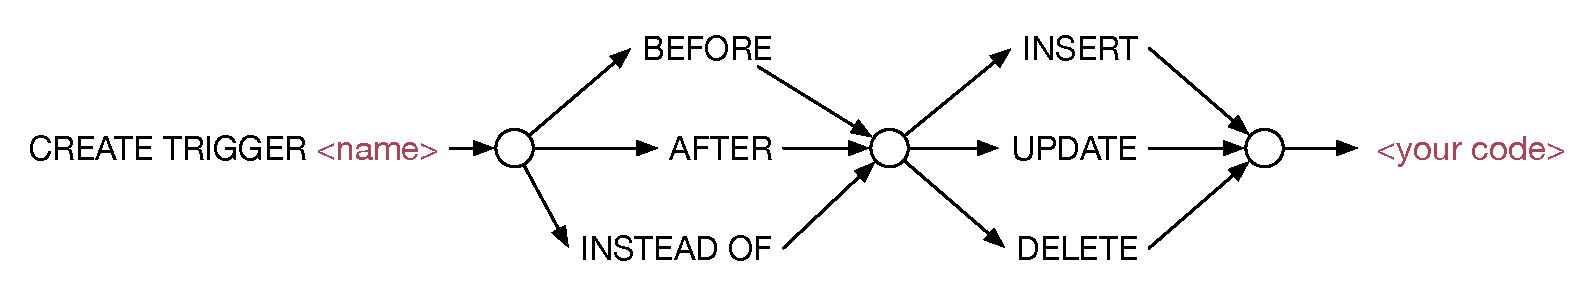
\includegraphics[width=\textwidth]{figures/create_trigger}
\end{center}

9 possible ``events'':\\
 - \lstinline[style=SQL]{BEFORE INSERT}: the code is executed before the new tuple is added;\\
 - \lstinline[style=SQL]{BEFORE UPDATE}: the code is executed before the tuple is changed;\\
 - ...

\vskip1em

\begin{block}{Triggers in SQLite}
\url{https://sqlite.org/lang_createtrigger.html}
\end{block}
\end{frame}

%
% ------------------------------------------------------------------------------
%

\begin{frame}

\begin{block}{`new' and `old' tuple variables}
There are two \underline{system-defined} tuple variables in a trigger:

\vskip0.5em

\lstinline[style=SQL]{-:new:-}:
\begin{itemize}[-,noitemsep,topsep=-0.5em]
 \item in an INSERT statement is the brand new tuple
 \item in an UPDATE statement is the modified tuple 
\end{itemize}

\vskip1em

\lstinline[style=SQL]{-:old:-}:
\begin{itemize}[-,noitemsep,topsep=-0.5em]
 \item in an UPDATE statement is the tuple before the change
 \item in a DELETE statement is tuple that will be removed 
\end{itemize}
 
\end{block}

\vfill

Different systems have different names for these tuple variables. We follow SQLite here.

\vskip1em

{Read up: \url{https://sqlite.org/lang_createtrigger.html}}
\end{frame}


%
% EXAMPLE TRIGGER -- saved to a box so we can reuse and shrink it
%
\newsavebox\triggerOne
\begin{lrbox}{\triggerOne}\begin{minipage}{0.875\textwidth}
\begin{lstlisting}[style=SQL,frame=single]
CREATE TRIGGER Constraint_1
BEFORE INSERT ON Cast
WHEN 10 <= (SELECT COUNT(*) FROM Cast c 
            WHERE -:new:-.title=c.title AND -:new:-.year=c.year)
BEGIN
    SELECT RAISE(ABORT, "Constraint #1 violated!");
END;
\end{lstlisting}%
\end{minipage}\end{lrbox}
%
% 
%

%
% ------------------------------------------------------------------------------
%

\begin{frame}

\textbf{Example constraint}: no movie can have more than 10 actors. Recall the foreign key \lstinline[style=SQL]{title,year} in \lstinline[style=SQL]{Cast} to the primary key in \lstinline[style=SQL]{Movie}.

\vskip2em

\begin{center}
\usebox\triggerOne
\end{center}


\end{frame}

%
% ------------------------------------------------------------------------------
%

\begin{frame}[fragile]

\vskip2em

\begin{columns}[onlytextwidth]
\begin{column}{0.4\textwidth}
\textbf{What is going on here?}
\vskip1em

The \lstinline[style=SQL]{WHEN} clause specifies the condition for the trigger to \emph{fire}\\
\end{column}
\begin{column}{0.55\textwidth}
\resizebox{\textwidth}{!}{\usebox{\triggerOne}}
\end{column}
\end{columns}

\vskip0.75em

The condition is checked for every tuple being inserted.

\vskip1em

The code between \lstinline[style=SQL]{BEGIN ... END;} is often called an \emph{SQL procedure} and defines what to do if the trigger \emph{fires} (in this case, abort the operation).

\vskip1em

The \lstinline[style=SQL]{RAISE(ABORT, "...")} command creates a runtime error that becomes an exception inside your code (or an error message in the console).
\end{frame}


\begin{frame}{\lstinline[style=SQL]!BEFORE! or \lstinline[style=SQL]!AFTER!?}

Most of the time, we want to check the constraint \lstinline[style=SQL]!BEFORE! the update is completed, and therefore we use that kind of trigger.

\vskip1em

Keep in mind that a trigger for \lstinline[style=SQL]!AFTER! an update runs after the database has already been modified, so we cannot use them to \emph{prevent} constraint violations. If you want to do that, the trigger must reverse the update that caused the violation.

Instead, \lstinline[style=SQL]!AFTER! triggers are normally used for automating tasks.
\begin{itemize}[-,topsep=-0.5em]
\item Ex: after an insertion into the ``orders'' table, if the inventory of an item is low, automatically purchase more items from the supplier.
\end{itemize}

\end{frame}


\begin{frame}[fragile]

\lstinline[style=SQL]{TRIGGER}s \alert{are not retroactive}!

\begin{itemize}[-]
\item When you add a trigger, the data already in the database is not checked for constraint violations! In our example, movies that had more than 10 actors at the time the \lstinline[style=SQL]{TRIGGER} is created will remain in the database.

\item When you add a constraint to a database that already has data, you must run queries to check, manually for violations of that constraint and deal with them accordingly.
\end{itemize}

\end{frame}


\begin{frame}[fragile]

\alert{Many constraints require multiple} \lstinline[style=SQL]{TRIGGER}s

\begin{itemize}[-]
\item You need to consider all combinations of insertions, deletions, and tuple updates that can cause which a constraint be violated and deal with them separately.

\item In our example, the number of actors in a movie can increase if we \lstinline[style=SQL]{UPDATE} a tuple already in the Cast table, changing its movie. To deal with that, we'd need another trigger, to run \lstinline[style=SQL]{BEFORE UPDATE} statements are done.
\end{itemize}


\end{frame}

\begin{frame}[fragile]{\lstinline[style=SQL]{STATEMENT} triggers}

Statement triggers can also be used to enforce table-level constraints:

\begin{lstlisting}[style=SQL]
CREATE TRIGGER Constraint_1B
BEFORE INSERT ON Cast REFERENCING (@NEW TABLE@) AS temp
(@FOR EACH STATEMENT@)
WHEN EXISTS (SELECT title,year 
             FROM Cast
             GROUP BY title, year
             HAVING (COUNT(*) > 10))
BEGIN
  SELECT RAISE(ABORT, "Constraint #1 violated!");
END;
\end{lstlisting}

\begin{block}{}
\alert{NOTE:} SQlite does not support \lstinline[style=SQL]{-:STATEMENT:-} triggers at the time of writing...
\end{block}
\end{frame}

%
% ------------------------------------------------------------------------------
%

\begin{frame}{Dealing with Constraint violations}

What should happen when an update statement would result in a constraint being \alert{violated}?

\begin{itemize}[-,noitemsep]
\item normally, we want to \textbf{abort} such update\\
 \item however, \underline{this may not be the default behavior}\footnote{SQLite allows the programmer to specify what to do for each individual \texttt{UNIQUE}, \texttt{NOT NULL} and \texttt{CHECK} constraint -- 
\url{https://sqlite.org/conflict.html}}
\end{itemize}

Note that some systems might allow \emph{some} of the updates to persist and prevent only the ones that violated the constraint. 

In our example, if we used a \lstinline[style=SQL]!(@ROW@)! trigger and attempted to insert three actors to a movie with 8 actors already, might mean that the first two actors are accepted and only the third is rejected.

\end{frame} 

\begin{frame}{Side effects?}

Can one trigger \emph{fire} another one? 
\begin{itemize}[-,noitemsep]
\item YES! If a trigger on table \lstinline[style=SQL]!A! contains insert statement into table \lstinline[style=SQL]!B! (note \lstinline[style=SQL]!A! and \lstinline[style=SQL]!B! can be the same), all constraints about table \lstinline[style=SQL]!B! are checked by the DBMS
\item in such cases, the execution environment (and the \emph{transient} tables) of the secondary trigger depends on the master trigger
\end{itemize}

\vskip1em

In a complex database with many business rules, even the simplest update can cause many triggers to fire and take a long time to complete.

\vskip1em \alert{Read up on} \url{https://www.sqlite.org/pragma.html\#pragma_recursive_triggers} to complete assignment 1.

\end{frame}

\begin{frame}[fragile]{Statement or Row triggers?}

SQL offers row-based and statement-based triggers to that the programmer can decide which events are best suited to enforce the business rule in their application. There is no clear cut distinction of when one should be used versus the other.

\vskip1em

The \emph{execution context} of a trigger (e.g., the values bound to the \lstinline[style=SQL]{new} and \lstinline[style=SQL]{old} variables) is defined by \emph{transient} tables which the DBMS must materialize.

\begin{itemize}[-,noitemsep]
\item Of course, these tables can be quite large, especially for statement triggers.
\end{itemize}
\end{frame}


\begin{frame}{Even more complex constraints?}

Some constraints can't be enforce per statement nor per row...

\alert{Example}: requiring every movie to have at least two actors (i.e., tuples in \lstinline[style=SQL]{Cast})?

\begin{itemize}[-,noitemsep]
\item Note that this means every time we insert a new movie (statement 1) we insert at least two actors (statement 2)...
\item But the foreign key constraint from \lstinline[style=SQL]!Cast! into \lstinline[style=SQL]!Movie! means we \textbf{cannot} insert an actor before we insert the movie!
\end{itemize}

\vskip2em

We cannot enforce such circularly-dependent constraints with the standard SQL constraint checking mechanisms. 

\end{frame}

\begin{frame}

Ways to deal with such constraints:
\begin{itemize}[-, noitemsep, topsep=-5pt]
\item \textbf{Delegate to the application}: \alert{problematic} when there are multiple applications (i.e., need to repeat code)
\item Define a \textbf{stored procedure} to insert all tuples at once\footnote{Stored procedures reside in the DBMS can can be used by all applications--avoiding code duplication.}
\end{itemize}

\vskip1em

Some DBMSs offer non-standard solutions, that are not specified by the SQL standard.

\begin{itemize}[-,noitemsep, topsep=-5pt]
\item PostgreSQL allows constraint checking to be \emph{deferred}, which implicitly allows the constraint to be checked once per complex transaction.
\item MS SQL server and Oracle allow the DBA to schedule the periodic execution of code (similar to a Unix \emph{cron job}) which can bed used to \textbf{detect} constraint violations.
\end{itemize}


\end{frame}

%
%
% Basic queries
%
%

\newsavebox\BasicSQLQuery
\begin{lrbox}{\BasicSQLQuery}
\begin{minipage}{0.9\textwidth}
%
% customize the text higlighter
%
\lstset{style=SQL,%
  keywords=[4]{table,value,expression,predicate,1,m,n,k},keywordstyle=[4]\ttfamily\bfseries\color{exampleColor},%
  keywords=[1]{SELECT,FROM,WHERE}}
  \begin{lstlisting}[style=SQL]
  SELECT value expression 1 [, ... [, value expression n]]
[ FROM table expression 1 [, ... [, table expression m ]]]
[ WHERE predicate 1 [ AND ... [ AND predicate k ]]]
\end{lstlisting}
\end{minipage}
\end{lrbox}

%
% ------------------------------------------------------------------------------
%


%
% ------------------------------------------------------------------------------
%

\section{Basic SQL\\{\small Syntax and Semantics}}

\begin{frame}[fragile]{Basic \lstinline[style=SQL]{SELECT ... FROM ... WHERE} queries}

Unlike the algebra, SQL is a very complex language that offers great freedom to the programmer---meaning the same query can be written in many different ways.\\
 
\begin{block}{}
CMPUT391 focuses on fundamental aspects of the language only, leaving out more esoteric constructs.
\end{block}

The basic SQL construct looks like this

\begin{center}
\fbox{\usebox\BasicSQLQuery}
\end{center}

Expressions inside square brackets are optional.
\end{frame}

%
% ------------------------------------------------------------------------------
%

\begin{frame}[fragile] %%%% VALUE EXPRESSIONS

As their name suggests, \textbf{value expressions} must compute atomic \emph{values} (as opposed to lists of values, tuples, etc.)

\vskip1em

\begin{columns}[onlytextwidth]
\begin{column}{0.5\textwidth}
A very common \emph{value expression} is just an attribute name.
\end{column}
\begin{column}{0.4\textwidth}
\begin{lstlisting}[style=SQL]
SELECT m.title
FROM Movie m;
\end{lstlisting}
\end{column}
\end{columns}

\begin{columns}
\begin{column}{0.5\textwidth}
But we can use operators and functions too.\footnotemark
\end{column}
\begin{column}{0.4\textwidth}
\begin{lstlisting}[style=SQL]
SELECT "title:{"||m.title||"}"
FROM Movie m;
\end{lstlisting}
\end{column}
\end{columns}

\begin{columns}
\begin{column}{0.5\textwidth}
In fact, anything that computes a single value is OK, including full SQL queries or expressions with them.
\end{column}
\begin{column}{0.4\textwidth}
\begin{lstlisting}[style=SQL]
SELECT 100 + (
        SELECT COUNT(*)
        FROM Movie m
       );
\end{lstlisting}
\end{column}

\end{columns}

\footnotetext{All examples follow SQLite notation; \lstinline[style=SQL]{||} means string concatenation}
\end{frame} 


%
% ------------------------------------------------------------------------------
%

\begin{frame}[fragile] %%%% TABLE EXPRESSIONS

\vskip1em

As their name suggests, \textbf{table expressions} must compute tables

\vskip1em

\begin{columns}[onlytextwidth]
\begin{column}{0.55\textwidth}
The most common \emph{table expression} is just a table name.\footnotemark
\end{column}
\begin{column}{0.375\textwidth}
\begin{lstlisting}[style=SQL]
SELECT m.title
FROM Movie AS m;
\end{lstlisting}
\end{column}
\end{columns}

\footnotetext{The \lstinline[style=SQL]{AS} $v$ clause creates a tuple variable $v$, making the query 
longer but \emph{more readable}. It is actually optional: \lstinline[style=SQL]{Movie m} would accomplish the same.}

\begin{columns}[onlytextwidth]
\begin{column}{0.375\textwidth}
But we can use full SQL ``sub-queries'' too.
\end{column}
\begin{column}{0.575\textwidth}
\begin{lstlisting}[style=SQL]
SELECT bmm.title
FROM (SELECT title, year FROM Cast
      WHERE actor="Bill Murray") AS bmm;
\end{lstlisting}
\end{column}
\end{columns}

\begin{columns}[onlytextwidth]
\begin{column}{0.425\textwidth}
In fact, anything that results in a table is OK.\footnotemark
\end{column}
\begin{column}{0.525\textwidth}
\begin{lstlisting}[style=SQL]
SELECT MAX(temp.b)
FROM (SELECT 1 AS a, 1 AS b
      UNION
      VALUES (2,2), (3,3)) AS temp;
\end{lstlisting}
\end{column}
\end{columns}

\footnotetext{\lstinline[style=SQL]{AS} can also be used to assign \emph{names} of columns and tables.}
\end{frame}


%
% ------------------------------------------------------------------------------
%

\begin{frame}[fragile] %%%% WHERE CLAUSES

As for the \textbf{predicates}...

\vskip1em

\begin{columns}[onlytextwidth]
\begin{column}{0.55\textwidth}
Most common: comparisons involving attributes and, possibly, built-in or user-defined functions.
\end{column}
\begin{column}{0.375\textwidth}
\begin{lstlisting}[style=SQL]
SELECT m.title
FROM Movie AS m
WHERE length(m.title) < 5;
\end{lstlisting}
\end{column}
\end{columns}

\begin{columns}[onlytextwidth]
\begin{column}{0.475\textwidth}
Using full SQL ``sub-queries'' is pretty common too.
\end{column}
\begin{column}{0.45\textwidth}
\begin{lstlisting}[style=SQL]
SELECT m.title 
FROM Movie m
WHERE m.imdb = (SELECT MAX(imdb)
                FROM Movie);
\end{lstlisting}
\end{column}
\end{columns}

\begin{columns}[onlytextwidth]
\begin{column}{0.375\textwidth}
And so is testing set membership.
\end{column}
\begin{column}{0.55\textwidth}
\begin{lstlisting}[style=SQL]
SELECT m.title
FROM Movie m
WHERE m.year IN (VALUES (1987),(1988));
\end{lstlisting}
\end{column}
\end{columns}

But there \lstinline[style=SQL]{EXISTS} many other kinds of useful predicates.
\end{frame}


\begin{frame}[fragile]{How do we execute a simple SQL query?}

Here's an algorithm that works (but is not the most efficient):

\begin{itemize}[-]
\item Go through each possible assignment of tuples to tuple variables tuple variable in the \lstinline[style=SQL]{FROM} clause.
\item For each such assignment, evaluate the \lstinline[style=SQL]{WHERE} clause.
\item If the value is \lstinline[style=SQL]{TRUE}, evaluate the expressions in the \lstinline[style=SQL]{SELECT} clause, and add them the to answer to the query.
\end{itemize}


Example:

\begin{lstlisting}[style=SQL]
SELECT g.film, g.year, m.director
FROM Guide g, Movie m
WHERE g.film = m.title AND g.year = m.year AND
      g.theater <> "Cineplex" AND m.imdb > 5 
\end{lstlisting}      



\end{frame}

\def\TableExpressions{\mathcal{T}}
\def\ValueExpressions{\mathcal{V}}
\def\Predicates{\mathcal{P}}
\def\VE{\mathit{ve}}
\def\TE{\mathit{te}}

%
% ------------------------------------------------------------------------------
%

\begin{frame}[fragile] %%%% BASIC SQL semantics
\label{algorithmForSQLTakeOne}

\vskip2em

\hspace*{-1em}\scalebox{0.8}{\begin{minipage}{1.35\textwidth}%

\textbf{Input:}  value expressions $\ValueExpressions=\{\VE_1,\dots,\VE_n\}$, table expressions $\TableExpressions=\{\TE_1,\ldots,\TE_m\}$,

\hspace*{5.125ex} predicates $\Predicates=\{p_1,\ldots,p_k\}$

\begin{algorithm}[H]
\begin{algorithmic}[1]
\If {$\TableExpressions = \emptyset$}
  \If {$\Predicates = \emptyset \ \ \  \text{OR}  \left(p_1 \wedge \cdots \wedge p_k\right)$} \Comment{no predicates OR all predicates are true}
      \State compute tuple $(ve_1, \ldots, ve_n)$ and add it to the \underline{result}
  \EndIf
\Else
    \ForEach {$te_i \in \TableExpressions$}
        \State $T_i \leftarrow $ table computed by $te_i$;
    \EndFor
    \ForEach {$t \in T_1 \times \cdots \times T_m$}
        \If {$\Predicates = \emptyset \ \ \  \text{OR}  \left(p_1(t) \wedge \cdots \wedge p_k(t)\right)$} \Comment{no predicates or $t$ satisfies all predicates}
            \State compute tuple $(ve_1, \ldots, ve_n)$ and add it to the \underline{result}
        \EndIf
    \EndFor
\EndIf
\end{algorithmic}
\caption{pseudocode to answer a \textbf{basic SQL query}}
\label{alg:seq}
\end{algorithm}
\end{minipage}}
\end{frame}

\begin{frame}[fragile]

The \lstinline[style=SQL]{WHERE} clause in a query can connect individual predicates using the logical connectives \lstinline[style=SQL]{AND}, \lstinline[style=SQL]{OR} and \lstinline[style=SQL]{NOT}, and one can use parenthesis to determine the precedence of the predicates and sub-expressions.

In a conjunctive query, the SQL processor will stop the evaluation of the \lstinline[style=SQL]{WHERE} clause once any predicate evaluates to \lstinline[style=SQL]{FALSE}. The processor will evaluate simpler predicates (e.g., comparisons involving constants) before evaluating the more complex ones (e.g., comparisons involving sub-queries).

Recall that logical expressions in SQL are three-valued\footnote{\url{https://en.wikipedia.org/wiki/Three-valued_logic}} (true, false, unknown). Combinations of tuples for which the \lstinline[style=SQL]{WHERE} evaluates to false or unknown are not used in the answer of the query.
\end{frame}

%
%
% Aggregation
%
%

%
% ------------------------------------------------------------------------------
%

\begin{frame}{Aggregation in SQL}

The SQL:1999 language is strictly more powerful than the ``standard'' relational algebra as discussed in the notes in the sense that every query expressible in the algebra is expressible in SQL, but not vice-versa.

\vskip1em

\begin{columns}[onlytextwidth]
\begin{column}{0.5\textwidth}
One feature of SQL that is not in the original algebra is the ability to compute \emph{aggregated values} (typically simple statistics) from \textbf{sets of tuples}
\end{column}

\begin{column}{0.45\textwidth}
\fbox{\begin{minipage}{\textwidth}
\small
\textbf{Set functions in SQL}\\
- \lstinline[style=SQL]{AVG()}: average (mean)\\
- \lstinline[style=SQL]{COUNT()}: number of values\\
- \lstinline[style=SQL]{MAX()}: largest value\\
- \lstinline[style=SQL]{MIN()}: smallest value\\
- \lstinline[style=SQL]{SUM()}: sum of values
\end{minipage}}
\end{column}
\end{columns}

Most DBMSs, including SQLite\footnote{\url{https://sqlite.org/lang_aggfunc.html}}, implement more set functions than the ones in the SQL:1999 standard.

\end{frame}


\newsavebox{\aggregationOnGuide}
\begin{lrbox}{\aggregationOnGuide}\begin{minipage}{0.5\textwidth}
\begin{lstlisting}[style=SQL]
SELECT theater, COUNT(*)
FROM Guide
GROUP BY theater
\end{lstlisting}
\end{minipage}
\end{lrbox}

%
% ------------------------------------------------------------------------------
%

\begin{frame}[fragile]

In an aggregation query, one value expression in the \lstinline[style=SQL]{SELECT} clause is a set function:

\vskip1em

\begin{center}
\begin{tikzpicture}[align=center,node distance=3cm,every node/.style={inner sep=0.5,outer sep=0.5}]
    \node (1) at (0,0) {\scalebox{0.75}{\usebox\CountStartOnGuideTable}};
    \node (2) [below of=1] {\scalebox{0.75}{\usebox\GuideTable}};
    \path[commutative diagrams/.cd, every arrow, every label]
        (2) edge node[swap] {~~\usebox\aggregationOnGuide} (1);   
\end{tikzpicture}
\end{center}

The \lstinline[style=SQL]{GROUP BY} clause tells SQL how to define the sets of tuples upon which to apply the set function: each (combination of ) unique value(s) defines a set.

\end{frame}


%
% ------------------------------------------------------------------------------
%

\begin{frame}[fragile]

To answer a simplified aggregation query:

\begin{center}
\lstset{style=SQL,%
  keywords=[4]{attribute,condition,table,value,expression,predicate,1,i,j,m,n,k},keywordstyle=[4]\ttfamily\bfseries\color{exampleColor},%
  keywords=[1]{SELECT,FROM,WHERE,GROUP,BY,HAVING}}
  \begin{lstlisting}[style=SQL]
  SELECT value expression 1 [, ... [, value expression n]]
[ FROM table expression 1 [, ... [, table expression m ]]]
[ WHERE predicate 1 [ AND ... [ AND predicate k ]]]
[ GROUP BY attribute 1 [, ... [, attribute i ]]]
[ HAVING condition 1 [ AND ... [ AND condition j ]]]
\end{lstlisting}
\end{center}


STEP 1: process the \lstinline[style=SQL]{FROM} and \lstinline[style=SQL]{WHERE} clauses (slide~\ref{algorithmForSQLTakeOne});

STEP 2: divide the tuples from STEP 1 into \emph{sets} according to the \lstinline[style=SQL]{GROUP BY} clause; if there is none, use all tuples as a single set;

STEP 3: if the \lstinline[style=SQL]{HAVING} clause is specified, discard sets of tuples that do not satisfy all conditions;

STEP 4: evaluate all expressions in the \lstinline[style=SQL]{SELECT} clause \underline{for each set separately}.
\end{frame}

\begin{frame}[fragile]

SQL supports a lot more in the \lstinline[style=SQL]{GROUP BY} and \lstinline[style=SQL]{HAVING} clauses than we cover in CMPUT391, including many operators for analytical data processing\footnote{\url{https://en.wikipedia.org/wiki/Online_analytical_processing}}, and value expressions.

For example, counting movies by decade:

\vskip1em

\begin{columns}[onlytextwidth]
\begin{column}{0.5\textwidth}
\begin{lstlisting}[style=SQL]
SELECT 10 * (year / 10), COUNT(*)
FROM Movie
GROUP BY year / 10
\end{lstlisting}
\end{column}

\begin{column}{0.35\textwidth}
\begin{lstlisting}[style=SQL]
1980 | 2
2000 | 1
2010 | 2
\end{lstlisting}
\end{column}
\end{columns}

Note that the value expression in the \lstinline[style=SQL]{SELECT} clause need not be the same as in the \lstinline[style=SQL]{GROUP BY} clause.

\end{frame}


\begin{frame}[fragile]{\lstinline[style=SQL]{DISTINCT} and \lstinline[style=SQL]{ORDER BY}}

\lstset{style=SQL,%
  keywords=[4]{attribute,condition,table,value,expression,predicate,1,i,j,m,n,k},keywordstyle=[4]\ttfamily\bfseries\color{exampleColor},%
  keywords=[1]{SELECT,FROM,WHERE,GROUP,BY,HAVING}}
  \begin{lstlisting}[style=SQL]
  SELECT [DISTINCT] value expression 1 [, ... [, value expression n]]
[ FROM table expression 1 [, ... [, table expression m ]]]
[ WHERE predicate 1 [ AND ... [ AND predicate k ]]]
[ GROUP BY attribute 1 [, ... [, attribute i ]]]
[ HAVING condition 1 [ AND ... [ AND condition j ]]]
[ ORDER BY -:col_no:- [ASC|DESC] ]
\end{lstlisting}

\lstinline[basicstyle=\ttfamily\bfseries\color{datatypeColor}]{DISTINCT} forces the DBMS to remove duplicates in the output. It is evaluated after all tuples are computed as before.

\lstinline[style=C,basicstyle=\ttfamily\bfseries\color{datatypeColor}]{ORDER BY} is executed last, even after \lstinline[basicstyle=\ttfamily\bfseries\color{datatypeColor}]{DISTINCT}, to sort the tuples in the output by the column specified (by is number from left to right).

\end{frame}


\section{Set/Bag Operations}

\begin{frame}{Set/bag operators in SQL}
SQL provides operators \lstinline[style=SQL]{UNION}, \lstinline[style=SQL]{INTERSECT}, and \lstinline[style=SQL]{EXCEPT} which are analogous to the algebra operators $\cup$, $\cap$ and $-$, respectively.

\vskip1em

Unlike the algebra, however, SQL is a \textbf{bag-oriented language}, 
meaning that duplicate tuples are allowed in a table;\footnote{Many textbooks use the term \textbf{relation} to mean a set of tuples, as in the algebra, and \textbf{table} to mean a bag of tuples (also called \emph{rows}) as in SQL}\\
 - bags are also called \emph{multisets}.

\vskip1em
 
You can tell the DBMS which ``version'' of the operators to use by appending the keyword \lstinline[style=SQL]{DISTINCT} (for sets) or \lstinline[style=SQL]{ALL} (for bags).
\end{frame}

%
% ------------------------------------------------------------------------------
%

\begin{frame}[fragile]
Suppose a tuple appears $m$ times in $R$ and $n$ times in $S$.

The following table shows the number of times it will appear in the result of each set/bag operator:

\vskip0.5em

\begin{minipage}{\textwidth}
\scriptsize\centering
\begin{tabular}{rll}
\hline
 & \textbf{DISTINCT} & \textbf{ALL}\\
R \textbf{UNION} S  & ~1 & $m+n$\\
R \textbf{INTERSECTION} S  & ~1 & $\min(m,n)$\\
R \textbf{EXCEPT} S  & ~0 & $\max(0,m - n)$\\
\hline
\end{tabular}
\end{minipage}

\vskip1em 

\begin{block}{In SQLite...}

...two or more simple SQL queries can be connected using \lstinline[style=SQL]{UNION} (which behaves as \lstinline[style=SQL]{UNION DISTINCT}), \lstinline[style=SQL]{UNION ALL}, \lstinline[style=SQL]{INTERSECT} and \lstinline[style=SQL]{EXCEPT}.

\vskip1em
Read \url{https://sqlite.org/lang_select.html}
\end{block}

\end{frame}

%
%
% negation
%
%

\section{Negation and Quantification}

%
% ------------------------------------------------------------------------------
%

\begin{frame}{Negation in SQL}

Queries that have only selections, projections, and joins, and for which the \lstinline[style=SQL]{WHERE} clause has only \lstinline[style=SQL]{AND} connectives form a class of queries called \underline{\emph{conjunctive queries}}.\footnote{More about this on the notes about the relational algebra}

If we also allow the use of disjunctions, either having \lstinline[style=SQL]{OR} connectives in the \lstinline[style=SQL]{WHERE} clause or using the \lstinline[style=SQL]{UNION} keyword, we have the class of \underline{\emph{positive queries}}.

These classes of queries are important and very well studied because most queries fall in either class and because they can be highly optimized by the DBMS.

However, these queries cannot express negation as in ``finding directors of movies \textbf{without} Bill Murray''.
\end{frame}

%
% ------------------------------------------------------------------------------
%


\newsavebox{\NEGATIONi}
\begin{lrbox}{\NEGATIONi}
\begin{lstlisting}[style=SQL]
SELECT director 
FROM Movie
EXCEPT
SELECT m.director
FROM Movie m, Cast c
WHERE m.title=c.title AND m.year=c.year AND c.actor="Bill Murray";
\end{lstlisting}
\end{lrbox}

\newsavebox{\NEGATIONii}
\begin{lrbox}{\NEGATIONii}
\begin{lstlisting}[style=SQL]
SELECT m.director 
FROM Movie m
WHERE NOT EXISTS(
    SELECT *
    FROM Movie m2, Cast c
    WHERE m2.title=c.title AND m2.year=c.year AND 
        c.actor="Bill Murray" AND m2.director=m.director);
\end{lstlisting}
\end{lrbox}

\newsavebox{\NEGATIONiii}
\begin{lrbox}{\NEGATIONiii}
\begin{lstlisting}[style=SQL]
SELECT director
FROM Movie
WHERE director NOT IN (
    SELECT m.director
    FROM Movie m, Cast c
    WHERE m.title=c.title AND m.year=c.year AND 
        c.actor="Bill Murray");
\end{lstlisting}
\end{lrbox}


\begin{frame}[fragile]
\label{negationSlideOne}
One way of achieving negation in SQL is by using the ``set difference'' \lstinline[style=SQL]{EXCEPT} operator between two queries:

\usebox{\NEGATIONi}

Another, perhaps more readable way:

\usebox{\NEGATIONii}
\end{frame}

%
% ------------------------------------------------------------------------------
%

\begin{frame}[fragile]
\label{negationSlideTwo}
Yet another way of expressing the query directors of movies without Bill Murray:

\usebox{\NEGATIONiii}

\end{frame}

%
% ------------------------------------------------------------------------------
%


\begin{frame}{Monotonicity}
\label{lab:monotonicity}

If a query is \emph{monotonic}\footnote{\url{https://en.wikipedia.org/wiki/Monotonic_query}}, \emph{adding} tuples to the database either leaves the result of the query unchanged or makes it grow.

All \alert{positive queries are monotonic}.
\begin{itemize}[-,topsep=-0.5em,noitemsep]
\item \textbf{Ex:} \lstinline[style=SQL]{SELECT DISTINCT year FROM Cast WHERE actor='Bill Murray'}
\item Adding a tuple to \lstinline[style=SQL]{Cast} cannot reduce the number of years in which Bill Murray had a movie.
\end{itemize}

\vskip2em

\begin{columns}[onlytextwidth]
\begin{column}{0.45\textwidth}
\blue{Negative queries are non-monotonic}: adding tuples might make the answer of the query smaller.
\end{column}
\begin{column}{0.6\textwidth}
\qquad\scalebox{0.75}{\usebox{\NEGATIONiii}}
\end{column}
\end{columns}

\vskip0.5em
\end{frame}

%
% ------------------------------------------------------------------------------
%



%
%
% ``Forall'' queries
%
%
\newsavebox\thereExistsExample
\begin{lrbox}{\thereExistsExample}
\begin{minipage}{0.44\textwidth}
\begin{lstlisting}[style=SQL]
SELECT m.director
FROM Movie m, Cast c
WHERE c.actor="Bill Murray"
      AND m.title=c.title
      AND m.year=c.year;
\end{lstlisting}
\end{minipage}
\end{lrbox}

%
% ------------------------------------------------------------------------------
%

\begin{frame}{Quantifiers in SQL}


\begin{columns}[onlytextwidth]
\begin{column}{0.65\textwidth}
Besides the algebra, SQL also borrows elements from Logic-based languages.

For example, tuple variables in SQL are \textbf{existentially quantified}.
\end{column}
\begin{column}{0.35\textwidth}
\scalebox{0.75}{\fbox{\usebox{\thereExistsExample}}}
\end{column}
\end{columns}

The query above seeking directors of movies with Bill Murray helps explain the concept.

Note that for a Movie $m$ to have its director in the answer, all we need is that \alert{\emph{there exists} a tuple $c$} in \lstinline[style=SQL]{Cast} such that $m$ and $c$ satisfy the conditions in the \lstinline[style=SQL]{WHERE} clause.

In this case, variable $c$ is \underline{existentially quantified} in the query.

\end{frame}

%
% ------------------------------------------------------------------------------
%

\begin{frame}
\vskip1em
What if we wanted directors who directed \textbf{all} movies in which Bill Murray appears?

In this case, for a Movie $m$ to have its director in the answer it must be the case that \alert{\textbf{all} tuples in \lstinline[style=SQL]{Cast}} that have Bill Murray as actor correspond to a movie directed by that director.

Now, variable $c$ is \underline{universally quantified} in the query.

\vskip1em

\begin{block}{Universal quantification via double negation}
SQL does not have specific notation for universal quantification.

\vskip1em

We use \underline{\textbf{double negation}} instead: the director of a Movie $m$ should appear in the answer if there is \alert{no} tuple $c$ in \lstinline[style=SQL]{Cast} such that $c$ has Bill Murray and $c$'s movie is \alert{not} directed by the director of $m$.
\end{block}

\end{frame}

\newsavebox\forAllExample
\begin{lrbox}{\forAllExample}
\begin{minipage}{0.44\textwidth}
\lstset{style=SQL,%
  keywords=[4]{NOT,EXCEPT},keywordstyle=[4]\ttfamily\bfseries\color{exampleColor},%
  keywords=[1]{SELECT,FROM,WHERE,EXISTS}}
\begin{lstlisting}[style=SQL]
SELECT m.director
FROM Movie m
WHERE NOT EXISTS (
            SELECT c.title, c.year
            FROM Cast c
            WHERE c.actor="Bill Murray"
            EXCEPT
            SELECT m2.title, m2.year
            FROM Movie m2
            WHERE m.director=m2.director
    );
\end{lstlisting}
\end{minipage}
\end{lrbox}


\begin{frame}[fragile]

Universal quantification via \underline{double negation}:

\vskip1em
\usebox{\forAllExample}
\end{frame}


%
%
% WITH CLAUSE --- Common Table Expressions
%
%

\section{Common Table Expressions}

%
% ------------------------------------------------------------------------------
%

\begin{frame}[fragile]{Table expressions}

The \lstinline[style=SQL]{FROM} clause in an SQL statement can contain \emph{any expression} that computes a table.

Example: ``which roles did Sigourney Weaver play in a top movie (rated 7 or higher)?''

\begin{lstlisting}[style=SQL]
SELECT c.role
FROM Cast c, 
     (SELECT title, year FROM Movie WHERE imdb >= 7) AS tm
WHERE c.title=tm.title AND c.year=tm.year AND
      c.actor="Sigourney Weaver";
\end{lstlisting}

In the query above, \lstinline[style=SQL]{AS} creates tuple variable \texttt{tm} (``top movie'').
\end{frame}

%
% ------------------------------------------------------------------------------
%

\begin{frame}[fragile]

We can make the query more readable by ``declaring'' all computed tables before the main query:

\vskip1em

\begin{lstlisting}[style=SQL]
WITH TopMovie(title, year) AS (
    SELECT title, year FROM Movie WHERE imdb >= 7
)
SELECT c.role
FROM Cast c, TopMovie tm
WHERE c.title=tm.title AND c.year=tm.year AND
      c.actor="Sigourney Weaver";
\end{lstlisting}

\vskip1em

\begin{block}{Common Table Expressions}
SQL queries declared inside \lstinline[style=SQL]{WITH} clauses are sometimes called \textbf{common table expressions} or CTEs
\end{block}

\end{frame}

%
% EXAMPLE SQL query reused in multiple slides
%
\newsavebox\QueryWithTwoCTEs
\begin{lrbox}{\QueryWithTwoCTEs}\begin{minipage}{.8\textwidth}
\begin{lstlisting}[style=SQL]
WITH TopMovie (title, year) AS (
	SELECT title, year FROM Movie WHERE imdb >= 7
),
RecentMovie (title, year) AS (
	SELECT title, year FROM Movie 
	WHERE strftime("%Y", year||"-01-01") >= 
        date("now","start of year")
)
SELECT c.role
FROM Cast c, TopMovie tm, RecentMovie rm
WHERE c.title=tm.title AND c.year=tm.year AND
      c.title=rm.title AND c.year=rm.year AND
      c.actor="Sigourney Weaver";
\end{lstlisting}\end{minipage}
\end{lrbox}

%
% ------------------------------------------------------------------------------
%

\begin{frame}[fragile]
\label{queryWithTwoCTEs}

We can have multiple CTEs in the same query:

\vskip1em
\scalebox{0.95}{\usebox\QueryWithTwoCTEs}

\end{frame}


%
% ------------------------------------------------------------------------------
%

\begin{frame}[fragile]

\begin{columns}[onlytextwidth]
\begin{column}{0.475\textwidth}
\textbf{What is going on here?\footnotemark}

\vskip1em 

- \lstinline[style=SQL]{strftime()} produces date/time values from a string;

\vskip0.5em 

- the double-pipe \lstinline[style=SQL]{||} operator concatenates two values (casting values to the proper types as needed);
\end{column}
\begin{column}{0.5\textwidth}
\scalebox{0.7}{\fbox{\usebox\QueryWithTwoCTEs}}
\end{column}
\end{columns}

- \lstinline[style=SQL]{strftime("%Y", year||"-01-01")} returns the date Jan. 1st of the year of the movie;\\ 
- \lstinline[style=SQL]{date("now","start of year")} returns Jan. 1st of the current year.

\footnotetext{The functions shown here are specific to SQLite! read up \url{https://sqlite.org/lang_datefunc.html}}

\end{frame}

%
%
% Recursion
%
%

%
% ------------------------------------------------------------------------------
%

\section{Recursive Queries}

\begin{frame}{Recursion in SQL}

There are many applications whose data consist of objects arranged in a \emph{graph}:
\begin{itemize}[-,noitemsep,topsep=-5pt]
\item cities connected by roads, rail lines or flights;
\item people connected by friendship, familial, or business relations;
\item courses connected by the pre-requisite relationship;
\item etc.
\end{itemize}

An important kind of query common to all these applications requires \emph{computing arbitrary paths} through these networks:
\begin{itemize}[-,noitemsep,topsep=-5pt]
\item finding all cities reachable from Edmonton by air with at most 2 connecting flights;
\item finding all actors directly or indirectly linked to Kevin Bacon.\footnote{\url{https://en.wikipedia.org/wiki/Six_Degrees_of_Kevin_Bacon}}
\end{itemize}

\end{frame}

%
% ------------------------------------------------------------------------------
%

\begin{frame} 
\label{language_influence_graph}
Example: graph of which languages influenced others.\footnote{Gathered browsing Wikipedia}

\vskip1em

\begin{columns}[onlytextwidth]
\begin{column}{0.4\textwidth}
\scalebox{0.8}{\usebox\LanguageInspiredTable}
\end{column}

\begin{column}{0.6\textwidth}
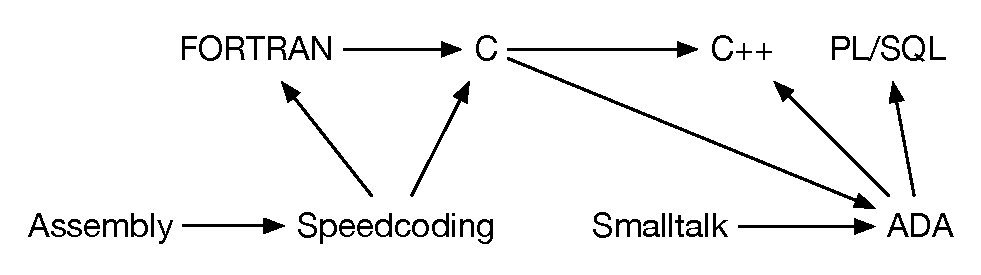
\includegraphics[width=\textwidth]{figures/recursion_language_inspired}
\end{column}
\end{columns}

\vskip1em

\begin{columns}[onlytextwidth]
\begin{column}{0.4\textwidth}
Which languages\\(directly or indirectly)\\influenced C++?
\end{column}

\begin{column}{0.6\textwidth}
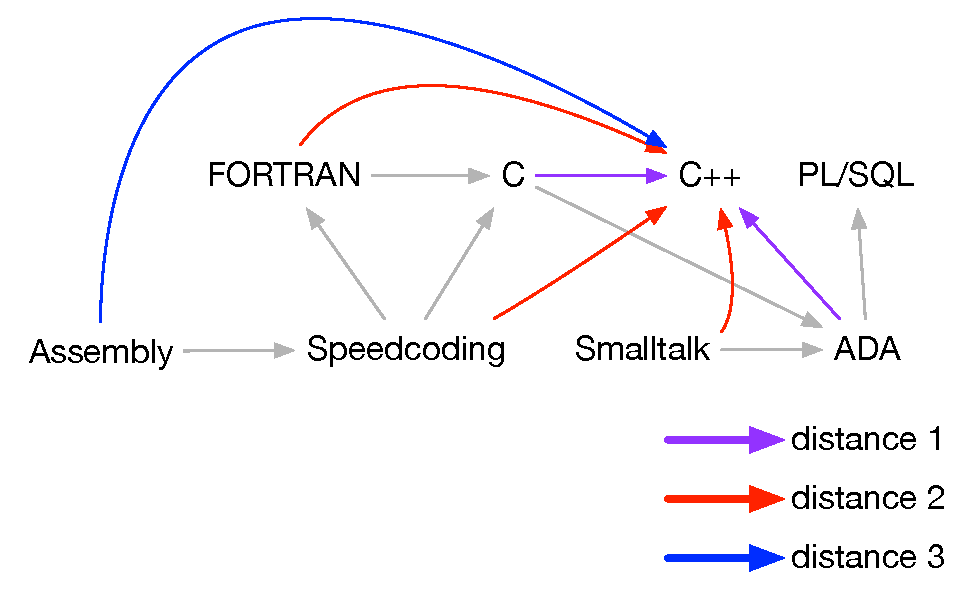
\includegraphics[width=\textwidth]{figures/recursion_language_inspired_CPP}
\end{column}
\end{columns}
\end{frame} 

%
% ------------------------------------------------------------------------------
%

\begin{frame}[fragile]

\begin{columns}[onlytextwidth]
\begin{column}{0.45\textwidth}
Distance=1: languages that \textbf{directly} influenced C++
\end{column}

\begin{column}{0.5\textwidth}
\begin{lstlisting}[style=SQL]
SELECT source
FROM Influence
WHERE target="C++"
\end{lstlisting}
\end{column}
\end{columns}


\begin{columns}[onlytextwidth]
\begin{column}{0.45\textwidth}
Distance=2: languages that influenced those that \textbf{directly} influenced C++
\end{column}

\begin{column}{0.5\textwidth}
\hspace*{2em}\begin{lstlisting}[style=SQL]
WITH dist1(language) AS (
  SELECT source FROM Influence 
  WHERE target="C++"
)
SELECT source FROM Influence
WHERE target IN 
  (SELECT language FROM dist1)
\end{lstlisting}
\end{column}
\end{columns}


\vskip2em

For this simple graph, the answer is the \textbf{union} of the queries above, as there is no language influencing C++ that is a distance 3 or higher...

\end{frame}


%
% ------------------------------------------------------------------------------
%

\begin{frame}[fragile]

But can we write a \textbf{single query} that works on \textbf{all graphs} regardless of the maximum distance?

\vskip1em

\begin{columns}[onlytextwidth]
\begin{column}{0.45\textwidth}
Distance=$n$: languages that influenced languages at distance $n-1$ from C++
\end{column}

\begin{column}{0.5\textwidth}
\hspace*{2em}\begin{lstlisting}[style=SQL]
WITH dist_n_1(language) AS (@???@)
SELECT source FROM Influence
WHERE target IN 
  (SELECT language FROM dist_n_1)
\end{lstlisting}
\end{column}
\end{columns}

\vskip1em

\begin{block}{``Standard'' SQL cannot compute arbitrary-length paths}
\begin{itemize}[-,noitemsep]
\item Each tuple in \lstinline[style=SQL]!Influence! is an edge in the graph
\item Each tuple variable can bind to a single tuple
\end{itemize}
\end{block}

\vskip1em

Therefore, a SQL query with $n$ tuple variables can only compute a path of length with at most $n$ edges.
\end{frame}

% \begin{frame}

% To find all languages that influenced C++ we need to proceed \textbf{recursively}:

% \vskip2em

% \begin{enumerate}[(1) ]
% \item Let $L$ be the set of all languages that directly influenced C++
% \item For every language $l_i$ that influenced another language $l_j \in L$
% \begin{itemize}[-]
% \item if $l_i$ isn't already in $L$; add it to $L$
% \end{itemize}
% \item Repeat step (2) until no more languages can be added to $L$.
% \end{enumerate}

% \end{frame}

%
% ------------------------------------------------------------------------------
%

\begin{frame}[fragile]

Finding languages that influenced C++ by taking the recursively computed \textbf{union}\footnote{Recall that in SQLite \lstinline[style=SQL]{UNION} defaults to \lstinline[style=SQL]{UNION DISTINCT}} of a query that finds languages that find direct influences to C++ and another that finds direct influences to those languages that influenced C++:

\vskip1em

\begin{lstlisting}[style=SQL]
WITH RECURSIVE Answer(language) AS (
  -- influenced C++ direclty:
  SELECT source FROM Influence WHERE target="C++"
UNION
  -- influenced some language that influenced C++:
  SELECT inf.source 
  FROM Influence inf, Answer A 
  WHERE inf.target = A.language
)
SELECT * FROM Answer;
\end{lstlisting}

\end{frame}

%
% ------------------------------------------------------------------------------
%

\newsavebox{\RECURSIVEexplained}
\begin{lrbox}{\RECURSIVEexplained}
\begin{minipage}{0.5\textwidth}
\begin{lstlisting}[style=SQL]
WITH RECURSIVE -:recursive_CTE:- AS (
  -:base query:-
UNION
  -:recursive query:-
)
\end{lstlisting}
\end{minipage}
\end{lrbox}

\begin{frame}[fragile]{SQL:199 Recursion}
Any recursive query must be defined as the \lstinline[style=SQL]{UNION} of two queries:

\begin{center}
\fbox{\usebox{\RECURSIVEexplained}}
\end{center}

The \lstinline[style=SQL]{-:base query:-} is non-recursive and must be defined over base tables only.

The \lstinline[style=SQL]{-:recursive query:-} must refer to the \lstinline[style=SQL]{-:recursive_CTE:-} exactly \textbf{once} and can refer to base tables as well. 
\end{frame}
%
% ------------------------------------------------------------------------------
%

\begin{frame}

\begin{center}
\fbox{\usebox{\RECURSIVEexplained}}
\end{center}

\vskip2em

Also: the \lstinline[style=SQL]{-:recursive query:-} must be \emph{monotonic} (recall Slide~\ref{lab:monotonicity}). 

In particular, it cannot use:
\begin{itemize}[-,topsep=-0.5em,noitemsep]
\item Aggregation;
\item \lstinline[style=SQL]{NOT EXISTS} with a subquery involving itself;
\item \lstinline[style=SQL]{EXCEPT} in which it is the right subquery.
\end{itemize}
\end{frame}



\begin{frame}{SQL:199 Recursion --- Semantics}

\begin{block}{The \emph{fixpoint} of an operator}
Suppose we start with a relation $R$, and that we repeatedly redefine it based on an operator $\oplus$ like so: 
\[R_1 = \oplus(R); \ R_2=\oplus(R_1); \ R_3 = \oplus(R_2); \ \cdots \]

\vskip0.5em

We reach a \emph{fixpoint} after $k$ applications of $\oplus$ when $R_{k+1}=R_k$ (that is, $\oplus$ no longer modifies the relation after $k$ applications)
\end{block}

SQL:1999 defines recursion in terms of fixpoints. 

More precisely, we start with a relation and continuously apply a suitably defined \lstinline[style=SQL]{UNION} operator until we reach a fixpoint.
\end{frame}

%
% ------------------------------------------------------------------------------
%

\begin{frame}[fragile]

Computing the influence on C++ with \emph{fixpoints}\\
- let $\text{Answer}_i$ be the answer at step $i$ and $\oplus$ be the recursive query

\vspace*{-1em}
\begin{center}
\small
\begin{align*}
\text{Answer}_0 =& \{\ \}\\
\text{Answer}_1 =& \oplus(\text{Answer}_0) = \{(\text{"C"}), (\text{"ADA"})\} \\
\text{Answer}_2 =& \oplus(\text{Answer}_1) = \{(\text{"C"}), (\text{"ADA"}), (\text{"FORTRAN"}), \\
&\ \ (\text{"Speedcoding"}), (\text{"Smalltalk"})\} \\
\text{Answer}_3 =& \oplus(\text{Answer}_2) = \{(\text{"C"}), (\text{"ADA"}), (\text{"FORTRAN"}), \\
& \ \ (\text{"Speedcoding"}), (\text{"Assembly"}), (\text{"Smalltalk"})\}\\
\text{Answer}_4 =& \oplus(\text{Answer}_3) = \text{Answer}_3
\end{align*}
\end{center}

We reach a \emph{fixpoint} at step 4 because no more languages are added to the answer.

\end{frame}


%
% ------------------------------------------------------------------------------
%


\begin{frame}{Generalizing Influence --- Graph Reachability}

\vskip0.5em

To find out ``which languages influenced \emph{an arbitrary} language $y$'' we need to find all languages $x$ such that $x\leadsto\text{y}$.

\vskip0.5em

\begin{block}{Reachability in a graph}
In an arbitrary graph, we say node $y$ is \alert{reachable} from node $x$ if there is a path $x\leadsto y$.
\end{block}

\vskip1em

\begin{columns}[onlytextwidth]
\begin{column}{0.65\textwidth}
\begin{block}{Computing \emph{reachability} with fixpoints}
- let the answer be the original graph

- let $\oplus$ be the union of the current graph and new edges formed by collapsing paths of length 2
\end{block}
\end{column}
~
\begin{column}{0.3\textwidth}
\resizebox{\textwidth}{!}{\includegraphics{figures/recursion_fixpoint.eps}}
\end{column}
\end{columns}
\end{frame}

\newsavebox\recursionCPPExample
\begin{lrbox}{\recursionCPPExample}
\begin{minipage}{0.8\textwidth}
\begin{lstlisting}[style=SQL]
WITH RECURSIVE Inspire(lang1, lang2) AS (
    SELECT source AS lang1, target AS lang2
    FROM Influence
  UNION
    SELECT edge.source, path.lang2
    FROM Inspire path, Influence edge
    WHERE edge.target=path.lang1
)
SELECT *
FROM Inspire;
\end{lstlisting}
\end{minipage}
\end{lrbox}

%
% ------------------------------------------------------------------------------
%


\begin{frame}

To find paths of arbitrary length recursively.

\vskip1em

\begin{enumerate}[(1) ]
\item Let $P$ be the set of all paths of length 1 (i.e., all edges in \lstinline[style=SQL]!Influence!).
\item For every pair of paths $p_1=(s_1,t_1) \in P, p_2=(s_2,t_2) \in P$ such that $p_1.t_1 = p_2.s_2$ (that is, $p_1$ ends in the language that $p_2$ starts):
\begin{itemize}[-]
\item if $p_3=(s_1,t_2)$ isn't already in $P$; add it to $P$
\end{itemize}
\item Repeat step (2) until no more new paths are added.
\end{enumerate}

\end{frame}


\begin{frame}[fragile]
\label{recursive_query_reachability}

Computing \emph{reachability} on the language influence graph:

\vskip1em

\begin{columns}[onlytextwidth]
\begin{column}{0.4\textwidth}

\scalebox{0.75}{\fbox{\usebox\recursionCPPExample}}

\end{column}
\begin{column}{0.35\textwidth}
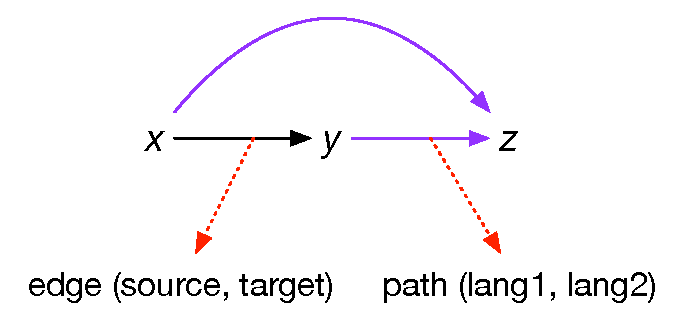
\includegraphics[width=1.25\textwidth]{figures/recursion_reachability_languages.eps}
\end{column}
\end{columns}

\vskip1em

To find the languages that influenced a language XYZ, filter the reachability graph to those edges incident on XYZ by adding the clause \lstinline[style=SQL]{WHERE lang2="XYZ"} to the query above.
\end{frame}

%
% ------------------------------------------------------------------------------
%

\begin{frame}[fragile]
\textbf{What is going on here?}

\vskip1em

\begin{columns}[onlytextwidth]
\begin{column}{0.5\textwidth}
\lstinline[style=SQL]{Inspire} is the ``answer'': the table representing the reachability graph.

\vskip1em

We start by adding all edges in \lstinline[style=SQL]{Influence} to the answer.
\end{column}

\begin{column}{0.5\textwidth}
\scalebox{0.65}{\fbox{\usebox\recursionCPPExample}}
\end{column}
\end{columns}

Then the \lstinline[style=SQL]{UNION} operator computes and adds \emph{new paths} $x\leadsto z$ whenever it can find an \emph{edge} $x\rightarrow y$ in \lstinline[style=SQL]{Influence} to extend a \emph{path} $y\leadsto z$ already in the reachability graph.

\vskip0.5em

\alert{IMPORTANT:} because \lstinline[style=SQL]{UNION} removes duplicates, we are guaranteed to reach a fixpoint!
\end{frame}

\newsavebox\boundedRecursion
\begin{lrbox}{\boundedRecursion}
\begin{minipage}{0.9\textwidth}
\begin{lstlisting}[style=SQL]
WITH RECURSIVE Inspire(lang1, lang2, (@len@)) AS (
    SELECT source AS lang1, target AS lang2, (@1 AS len@)
    FROM Influence
  UNION
    SELECT edge.source, path.lang2, (@path.len+1@)
    FROM Inspire path, Influence edge
    WHERE edge.target = path.lang1 AND (@path.len < 5@)
)
SELECT *
FROM Inspire;
\end{lstlisting}
\end{minipage}
\end{lrbox}

%
% ------------------------------------------------------------------------------
%

\begin{frame}[fragile]

What if we want only paths of length up to $k$?\\
 - we could take the union of queries computing paths of length $1, 2, \ldots, k$;\\
 - \textbf{or} we can \textbf{impose a bound} on the recursion.

\vskip1em

Example ($k=5$): 
\usebox\boundedRecursion
\end{frame}

\newsavebox\recursiveQueryOnGraphWithCycles
\begin{lrbox}{\recursiveQueryOnGraphWithCycles}
\begin{minipage}{0.675\textwidth}\begin{lstlisting}[style=SQL]
WITH RECURSIVE Path(begin_, end_, len) AS (
    SELECT source, target, 1
    FROM Edge
  UNION
    SELECT e.source, p.end_, p.len+1
    FROM Path p, Edge e
    WHERE e.target = p.begin_ AND p.len < 5
)
SELECT *
FROM Path;
\end{lstlisting}\end{minipage}
\end{lrbox}

%
% ------------------------------------------------------------------------------
%

\begin{frame}[fragile]
\label{recursionWithCycles}
\textbf{What if there are cycles in the graph?}

\begin{figure}
\begin{subfigure}{0.3\textwidth}
\usebox\GraphWithCycle
\end{subfigure}
~~~~~
\begin{subfigure}{0.6\textwidth}
\scalebox{0.75}{\fbox{\usebox\recursiveQueryOnGraphWithCycles}}
\end{subfigure}
\end{figure}

We get many ``copies'' of the path $n_1\leadsto n_2$ with different lengths:\\
 - length 1: $n_1\rightarrow n_2$ \\
 - length 3: $n_1\rightarrow n_2 \rightarrow n_1 \rightarrow n_2$ \\
 - length 5: $n_1\rightarrow n_2 \rightarrow n_1 \rightarrow n_2 \rightarrow n_1 \rightarrow n_2$ \\

\end{frame}


\begin{frame}[fragile]{Recursion on Numbers}

Of course, recursion in SQL is not restricted to graph traversals. In fact, one can express many familiar recursive computations in SQL.

\textbf{Example:} the sum of the first $N=100$ non-negative numbers:

\vskip1em
\begin{center}
\begin{minipage}{0.75\textwidth}
\begin{lstlisting}[style=SQL]
WITH RECURSIVE c(n) AS (
   SELECT 1
  UNION
    SELECT n+1 FROM c WHERE n<100
) SELECT SUM(n) 
FROM c;
\end{lstlisting}
\end{minipage}
\end{center}

\end{frame}


%
% ------------------------------------------------------------------------------
%

\begin{frame}{DBMS support for recursive SQL} %%% RECURSIVE SQL IN OTHER SYSTEMS

The SQL:1999 standard defined recursion in terms of the fixpoint operator on \textbf{common table expressions} as discussed here.

In the 1980's, Oracle introduced a different syntax and mechanism for recursion 
through so-called \emph{hierarchical queries}.\footnote{\tiny\url{https://en.wikipedia.org/wiki/Hierarchical_and_recursive_queries_in_SQL}} 

Today, both Oracle and IBM support both forms of recursion, while Microsoft's SQL Server supports the SQL:1999.

In the open-source world, besides SQLite, PostgreSQL\footnote{\tiny\url{https://www.postgresql.org/docs/current/static/queries-with.html}}, Firebird\footnote{\tiny\url{http://www.firebirdsql.org}}, and CUBRID\footnote{\tiny\url{http://www.cubrid.org}} support the SQL:1999 standard.
\end{frame} %%% RECURSIVE SQL IN OTHER SYSTEMS

%
%
% The big picture
%
%

% \section{Equivalence Between the ``Standard SQL'' and the Algebra}

% %!TEX root = lec02_sql.tex

%
% ------------------------------------------------------------------------------
%

\begin{frame}{SQL Equivalence with the Relational Algebra}

Although very different in many respects, SQL and the algebra share many commonalities. In fact, we can write in the algebra many queries that are also expressible in SQL.

This is a good thing because there is an efficient (and easy to optimize) algorithm to compute answers to algebra expressions. 

Thus, we can answer a SQL query by: (1) translating it into an equivalent algebra expression; and (2) evaluating that expression efficiently.

\textbf{This is in fact what most DBMSs do!}

CMPUT391 is not a theory course, so we will not prove any equivalence results. Instead, only some hints are given.

\end{frame}


%
% ------------------------------------------------------------------------------
%

\newsavebox\algebraBasicSelectFromWhere
\savebox{\algebraBasicSelectFromWhere}{
    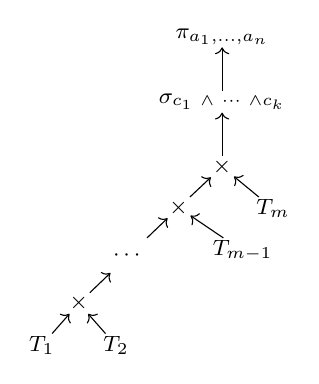
\begin{tikzpicture}[align=center,node distance=0.825cm,every node/.style={inner sep=0.5,outer sep=0.5,font=\footnotesize}]
    \node (P1) at (0,0) {$\pi_{a_1,\ldots,a_n}$};
    \node (P2) [below of=P1] {$\sigma_{c_1\ \wedge\ \cdots\ \wedge c_k}$};
    \node (P3) [below of=P2] {$\times$};
    \node (P4) [below left=0.25cm and 0.25cm of P3] {$\times$};
    \node (P5) [below right=0.25cm and 0.25cm of P3] {$T_m$};
    \node (P6) [below right=0.25cm and 0.25cm of P4] {$T_{m-1}$};
    \node (P7) [inner sep=4,below left=0.25cm and 0.125cm of P4] {$\cdots$};
    \node (P8) [below left=0.25cm and 0.125cm of P7] {$\times$};
    \node (P9) [below left=0.25cm and 0.125cm of P8] {$T_1$};
    \node (P10) [below right=0.25cm and 0.125cm of P8] {$T_2$};
    \path[commutative diagrams/.cd, every arrow, every label]
        (P2) edge node {} (P1)
        (P3) edge node {} (P2)
        (P4) edge node {} (P3)
        (P5) edge node {} (P3)
        (P6) edge node {} (P4)
        (P7) edge node {} (P4)
        (P8) edge node {} (P7)
        (P9) edge node {} (P8)
        (P10) edge node {} (P8);
\end{tikzpicture}%
}


\begin{frame}[fragile] %%%% equivalence of SQL and algebra
\label{AlgebraSQLEquivalencePartI}
\vskip1em
\begin{BOX}{Algebra and SQL equivalence -- take 1}
It should now be obvious that one can easily write an algebra expression equivalent to a SQL query where:\\
 - value expressions are attribute names\\
 - table expressions are base tables\\
 - predicates are comparisons involving attributes and/or constants
\end{BOX}

\vskip1em

\begin{columns}%[onlytextwidth]
\begin{column}{0.275\textwidth}
\begin{lstlisting}[style=cmput391,language=SQL,escapeinside={(*}{*)},frame=single]
SELECT (*$a_1, a_2, \ldots, a_n$*)
FROM (*$T_1, T_2, \ldots, T_m$*)
WHERE (*$c_1, c_2, \ldots, c_k$*)
\end{lstlisting}
\end{column}

\begin{column}{0.45\textwidth}
\scalebox{1.1}{\usebox\algebraBasicSelectFromWhere}
\end{column}
\end{columns}
\end{frame}


%
% EXAMPLE SQL QUERY FOR NEXT SLIDE
%
\newsavebox\SQLqueryBMM
\begin{lrbox}{\SQLqueryBMM}
\begin{minipage}{0.44\textwidth}
\begin{lstlisting}[style=SQL]
SELECT m.director
FROM Movie m, 
  (SELECT title, year 
   FROM Cast
   WHERE actor='Bill Murray'
  ) AS bmm
WHERE m.year=bmm.year 
  AND m.title=bmm.title;
\end{lstlisting}
\end{minipage}
\end{lrbox}

%
% ------------------------------------------------------------------------------
%

\begin{frame}[fragile]
\label{AlgebraSQLEquivalencePartII}
\vskip1em
\begin{BOX}{Algebra and SQL equivalence -- take 2}
 - Renaming in the algebra ($\rho$) can be used to handle SQL's \lstinline{AS} clauses

 \vskip0.5em

 - Table expressions that look like the ``simple SQL'' in slide~\ref{AlgebraSQLEquivalencePartI} can be expressed as ``sub-queries'' under the main $\times$ operator
\end{BOX}

\vskip1em

\begin{columns}%[onlytextwidth]
\begin{column}{0.275\textwidth}
\scalebox{0.75}{\fbox{\usebox\SQLqueryBMM}}
\end{column}
\begin{column}{0.6\textwidth}
\scalebox{1.1}{%
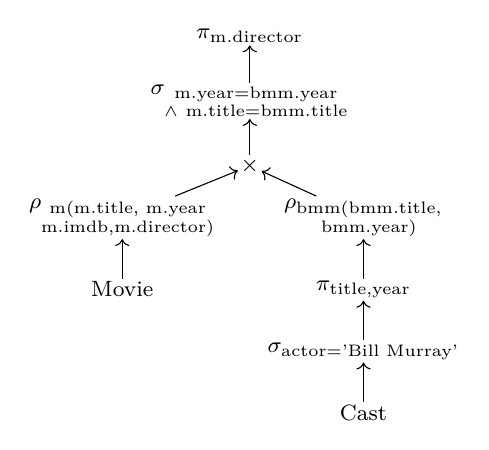
\begin{tikzpicture}[align=center,node distance=0.825cm,every node/.style={inner sep=0.5,outer sep=0.5,font=\footnotesize}]
    \node (P1) at (0,0) {$\pi_{\text{m.director}}$};
    \node (P2) [below of=P1] {$\sigma_{\substack{\text{m.year=bmm.year}\\\wedge\ \text{m.title=bmm.title}}}$};
    \node (P3) [below of=P2] {$\times$};
    \node (P4) [below right=0.25cm and 0.25cm of P3] {$\rho_{\substack{\text{bmm(bmm.title,}\\%
           \text{bmm.year)}}}$};
    \node (P5) [below left=0.25cm and 0.25cm of P3] {$\rho_{\substack{\text{m(m.title, m.year}\\
           \text{m.imdb,m.director)}}}$};
    \node (P6) [below=0.5cm of P4] {$\pi_{\text{title,year}}$};           
    \node (P7) [below=0.5cm of P6] {$\sigma_{\text{actor='Bill Murray'}}$};
    \node (P8) [below=0.5cm of P7] {Cast};
    \node (P9) [below=0.5cm of P5] {Movie};
    \path[commutative diagrams/.cd, every arrow, every label]
        (P2) edge node {} (P1)
        (P3) edge node {} (P2)
        (P4) edge node {} (P3)
        (P5) edge node {} (P3)
        (P6) edge node {} (P4)
        (P7) edge node {} (P6)
        (P8) edge node {} (P7)
        (P9) edge node {} (P5);
\end{tikzpicture}%
}
\end{column}
\end{columns}
\end{frame}

%
% ------------------------------------------------------------------------------
%

\begin{frame}[fragile]

\begin{BOX}{What about aggregation?}

Most textbooks give an ``extended algebra'' with an operator \[\gamma_{\text{<grouping>,fn()}}(R)\]

The \lstinline{GROUP BY} clause goes into ``grouping'' and fn() is the set function. The \lstinline{HAVING} clause are handled with a selection.
\end{BOX}

\vskip1em

\begin{columns}[onlytextwidth]
\begin{column}{0.3\textwidth}
\begin{lstlisting}[style=SQL]
SELECT theater, COUNT(*) 
FROM Guide
WHERE start > 1100
GROUP BY theater
HAVING COUNT(*) > 4
\end{lstlisting}
\end{column}
\begin{column}{0.4\textwidth}
\scalebox{1}{
     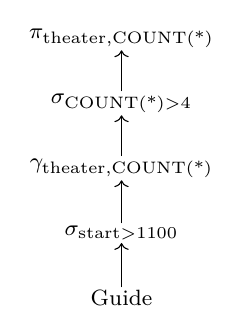
\begin{tikzpicture}[align=center,node distance=0.825cm,every node/.style={inner sep=0.5,outer sep=0.5,font=\footnotesize}]
    \node (P1) at (0,0) {$\pi_{\text{theater},\text{COUNT(*)}}$};
    \node (P2) [below of=P1] {$\sigma_{\text{COUNT(*)}>4}$};
    \node (P3) [below of=P2] {$\gamma_{\text{theater},\text{COUNT(*)}}$};
    \node (P4) [below of=P3] {$\sigma_{\text{start}>1100}$};
    \node (P5) [below of=P4] {\lstinline{Guide}};
    \path[commutative diagrams/.cd, every arrow, every label]
        (P2) edge node {} (P1)
        (P3) edge node {} (P2)
        (P4) edge node {} (P3)
        (P5) edge node {} (P4);
\end{tikzpicture}%
}
\end{column}
\end{columns}
\end{frame}


\begin{frame}

\begin{BOX}{What about recursion?}
Recursion is normally left out of the algebra.
\end{BOX}

\vskip3em

\begin{BOX}{What about universal quantification?}
Many textbooks add a \textbf{division} operator to the algebra, specifically to compute ``for all'' queries. However, most relational engines do not use that operator in query plans.
\end{BOX}

\end{frame}

%
% ------------------------------------------------------------------------------
%

% \begin{frame}

% Abridged relationship between classes of queries and relational languages

% 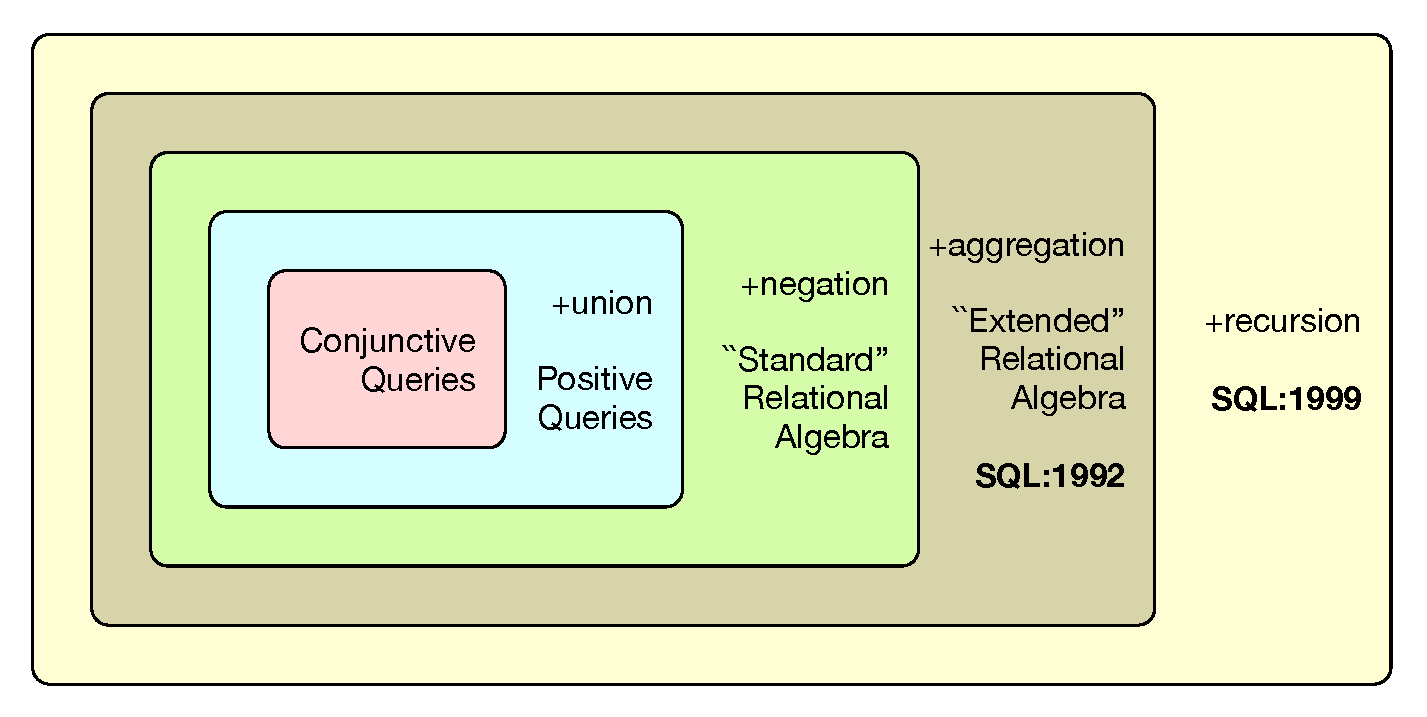
\includegraphics[width=\textwidth]{figures/algebra_SQL}

% \end{frame}

% %
% %
% % Other relational languages
% %
% %


\end{document}